% !TeX program = XeLaTeX

\documentclass[aspectratio=169]{beamer}
\usepackage[T1]{fontenc}
\usepackage[ngerman]{babel}
\usetheme[logo=img/zeeman_splitting2.png, faculty=ped]{fibeamer}


\include{preamble}
%\usepackage[latin1]{inputenc}

\usepackage{booktabs}
\usepackage{siunitx}
\sisetup{seperr}
\sisetup{expproduct=\cdot,per=frac,fraction=nice}

\makeatletter
\setlength\fibeamer@lengths@logowidth{10em}
\setlength\fibeamer@lengths@logoheight{10em}
\newenvironment{myframe}[2][\insertsection]{%
    \addtobeamertemplate{frametitle}{\vspace{.2cm}\hskip-.7\beamer@leftmargin\scriptsize \hspace*{.75cm}\textcolor{gray!50!white}{#1}\vspace*{-.8cm}}{}
    \begin{frame}{#2}%
}{%
    \end{frame}
}
\tikzset{
  invisible/.style={opacity=0},
  visible on/.style={alt={#1{}{invisible}}},
  alt/.code args={<#1>#2#3}{%
    \alt<#1>{\pgfkeysalso{#2}}{\pgfkeysalso{#3}} % \pgfkeysalso doesn't change the path
  },
}

\makeatother
\definecolor{fibeamer@lightOrange}{HTML}{329cac}
\definecolor{fibeamer@orange}{HTML}{228c9c}
\setbeamertemplate{caption}[numbered]

%% These macros specify information about the presentation
\title{FP F44 - Zeeman-Effekt} %% that will be typeset on the
\author{Patrick Nisble, David Bubeck}

% testing
\newcommand{\var}{\newcommand}

% vars
\var\inclineUp{\SI{39.461+-2.198}{\milli\tesla\per\ampere}}
\var\inclineDown{\SI{38.874+-2.192}{\milli\tesla\per\ampere}}

\var\magnetonOneVal{9.956+-0.414}
\var\magnetonOne{\SI{\magnetonOneVal e-24}{\joule\per\tesla}}
\var\magnetonTheoVal{9.274}
\var\magnetonTheo{\SI{\magnetonTheoVal e-24}{\joule\per\tesla}} % 0099942
\var\magnetonTwoVal{8.138+-0.271}
\var\magnetonTwo{\SI{\magnetonTwoVal e-24}{\joule\per\tesla}}

\var\lambdaCdTheoVal{643.847}
\var\lambdaCdTheo{\SI{\lambdaCdTheoVal}{nm}}
\var\lambdaCdVal{643.927+-0.571}
\var\lambdaCd{\SI{\lambdaCdVal}{\nano\metre}}
\var\lambdaTh{\SI{652.250}{nm}}
\var\lambdaXeVal{652.151}
\var\lambdaXe{\SI{\lambdaXeVal}{nm}}
\var\lambdaUkVal{652.253+-0.269}
\var\lambdaUk{\SI{\lambdaUkVal}{nm}}
\var\pxCd{\SI{547.945+-4.310}{px}}

\frenchspacing
\begin{document}
  \frame{\maketitle}
  \begin{frame}<beamer>
    \frametitle{Outline}
    \tableofcontents[hideallsubsections]
  \end{frame}

  \AtBeginSection[]{% Print an outline at the beginning of sections
  \begin{frame}<beamer>
    \frametitle{Outline - \insertsection}
    \tableofcontents[currentsection, hideothersubsections]
  \end{frame}}


  % !TeX root = ../pres.tex

\section{Einleitung}


    \subsection{Grundlagen}
        \begin{myframe}{\subsecname}
            Beschreibung des Zeeman-Effekt in einer Näherung:
            \begin{itemize}
                \item Drehimpuls des Elektrons: \\ $\vec{l} = \vec{r} \times \vec{p} = m_e \cdot v \cdot \vec{n}$
                \item Elektron kann mit einem Strom $ I $ und magnetischen Moment $\mu_{l}$ beschrieben werden. \\
                    $\vec{\mu_{l}} = \underbrace{I}_{- e \frac{v}{2 \pi r}} \cdot \underbrace{\vec{A}}_{\text{Flächenvektor zur Orbitfläche}} = \frac{evr}{2} \vec{n}$
                \item Interaktion mit externen Magnetfeld und dem magnetischen Moment ergibt sich Änderung der potentiellen Energie
                \item mit $\vec{l}$ quantisiert (d.h. $l_z = m_l \cdot \hbar$) und $\vec{B} \parallel \vec{l}$ erhält man
                \begin{itemize}
                    \item[] $\Delta E_{pot} = \frac{e \cdot \hbar}{2m_e} \cdot m_l \cdot B = \mu_B \cdot m_l \cdot B $
                    \begin{itemize}
                        \item[] $\mu_{B}$ : Bohr'sche Magneton
                    \end{itemize}
                \end{itemize}
            \end{itemize}
        \end{myframe}

        \begin{myframe}{\subsecname}
            Atome mit mehreren Elektronen:
            \begin{itemize}
                \item $\vec{L} \vec{S}$ - Kopplungsnäherung
                \item Gesamtdrehimpuls $\vec{J} = \vec{L} + \vec{S}$
                \begin{itemize}
                    \item[] wobei:
                    \item $\vec{L} = \sum_i \vec{l_i}$
                    \item $\vec{S} = \sum_i \vec{s_i}$
                \end{itemize}
                \item $\Delta E_{pot} = \mu_B \cdot B \cdot M_J \cdot g_J $
                \begin{itemize}
                    \item mit dem Landé - Faktor $g_{J} = 1 + \frac{J(J + 1) + S(S + 1) - L(L + 1)}{2J(J + 1)}$
                \end{itemize}
            \end{itemize}
            \begin{align*}
              S = 0 \text{ und } g_{J} = 1 &\rightarrow \text{ \textbf{normaler} Zeeman - Effekt} \\
              \text{ ansonsten } &\rightarrow \text{ \textbf{anomaler} Zeeman - Effekt}
            \end{align*}
        \end{myframe}



    \subsection{Auswahlregeln}
        \begin{myframe}{\subsecname}
            % \begin{itemize}
                % \item Impuls-, Drehimpulserhaltung
                % \item Symmetrieeigenschafen
                % \item $\vec{M_{ik}} = e \int \Psi_i^* \; \vec{r} \; \Psi_k \; dV \neq 0 $
                \vspace{-.7cm}
                \begin{align*}
                    \vec{M_{ik}} = e \int \Psi_i^* \; \vec{r} \; \Psi_k \; dV \neq 0
                \end{align*}
                \vspace{-.3cm}
                \begin{columns}
                    \begin{column}{0.48\textwidth}
                    Auswahlregeln:
                        \begin{itemize}
                            \item $\Delta M_J = M_{J,i} - M_{J,k} = 0, \pm 1 $
                            \item $\Delta L = \pm 1 \text{ und } \Delta S = 0 $
                            \item $\Delta M_J = \pm 1 \; \widehat{=}$ zirkular polarisierendem Licht mit Phasenverschiebung $\frac{\pi}{2}$ \\ ($\sigma$ - Übergang)
                            \item $\Delta M_J = 0 \; \widehat{=}$ linear polarisierendem Licht ($\pi$ - Übergang)
                        \end{itemize}
                    \end{column}
                    \begin{column}{0.48\textwidth}
                        \begin{figure}
                            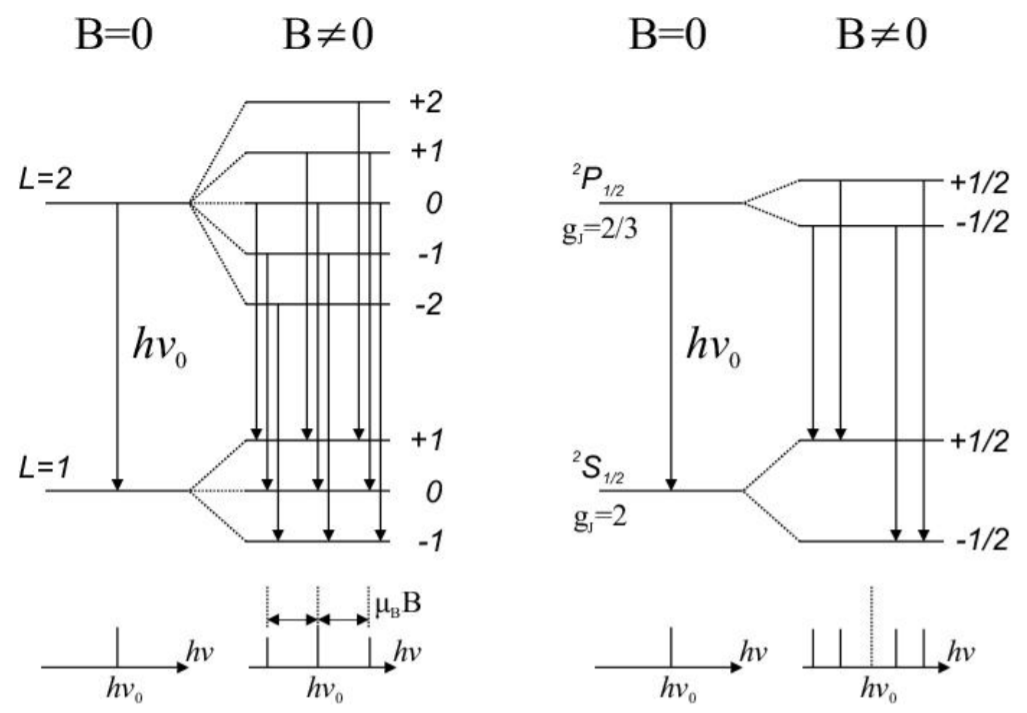
\includegraphics[width=0.8\linewidth]{img/zeemanSplittingScheme.png}
                            \caption{Zeeman - Effekt Thermschema, Quelle: FP 44 Versuchsscript}
                            \label{zeemanEffektScheme}
                        \end{figure}
                    \end{column}
                \end{columns}
                % \item $\Delta M_J = \pm 1 \; \widehat{=}$ zirkular polarisierendem Licht mit Phasenverschiebung $\frac{\pi}{2}$ \\ ($\sigma$ - Übergang)
                % \item $\Delta M_J = 0 \; \widehat{=}$ linear polarisierendem Licht ($\pi$ - Übergang)
            % \end{itemize}

        \end{myframe}



    \subsection{Lummer - Gehrcke Platte}
        \begin{myframe}{\subsecname}
            \begin{figure}
                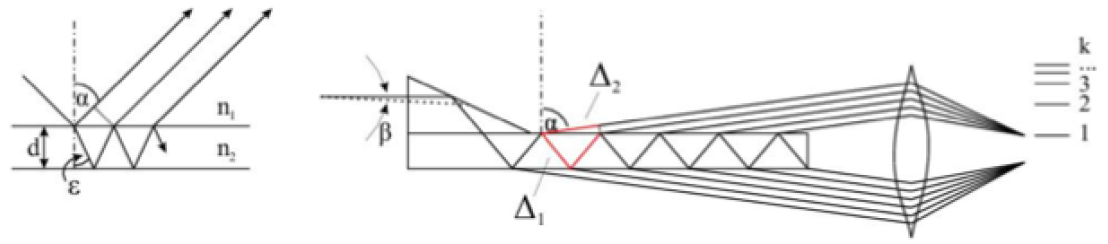
\includegraphics[width=0.8\linewidth]{img/lummerGehrckePlate.png}
                \caption{Lummer - Gehrcke Platte, Quelle: FP 44 Versuchsscript}
                \label{lummerGehrckePlate}
            \end{figure}
            \begin{itemize}
                \item Licht wird nahe der Totalreflexion reflektiert
                \item Hohe Auflösung durch Interferenz der ausfallenden Lichtstrahlen mit Gangunterschied
                    \begin{equation*}
                        \Delta \approx 2d \cdot \sqrt{n^2 - 1} = k \lambda \text{, } k \in \mathbb{N} \qquad \qquad \text{für } \alpha \sim 90^{\circ}
                    \end{equation*}
            \end{itemize}
        \end{myframe}



    \subsection{Czerny - Turner Spektrometer}
        \begin{myframe}{\subsecname}
            \begin{figure}
                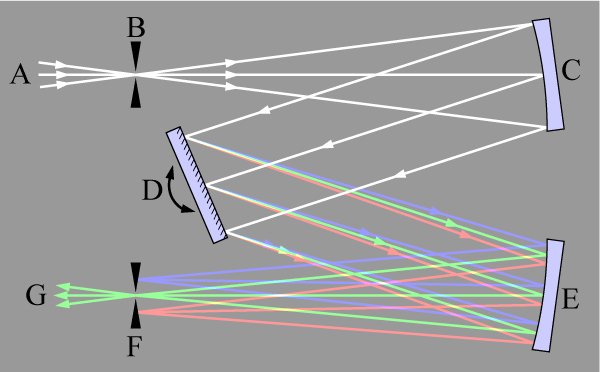
\includegraphics[width=0.6\linewidth]{img/czernyTurnerSpectrometer_Wikipedia.png}
                \caption{Aufbau eines Czerny - Turner Spektrometer, Quelle: https://de.wikipedia.org/wiki/Monochromator}
                \label{czernyTurnerSpektrometer}
            \end{figure}
        \end{myframe}

  % !TeX root = ../pres.tex

\section{Versuchsaufbau}

    \subsection{1. Versuchsteil - Spektroskopie des Zeeman - Effekts}
        \begin{myframe}{\subsecname}
            \begin{itemize}
                \item Verwendung der Lummer - Gehrcke Platte zur Beobachtung des Zeeman - Effekts
                \item Beobachtung der Polarisationseigenschaften mit Hilfe von Polarisationsfiltern und $\frac{\lambda}{4}$ Filter
                \item Bestimmung des Bohr'schen Magnetons
            \end{itemize}
        \end{myframe}

        \begin{myframe}{\subsecname}
            \begin{figure}
                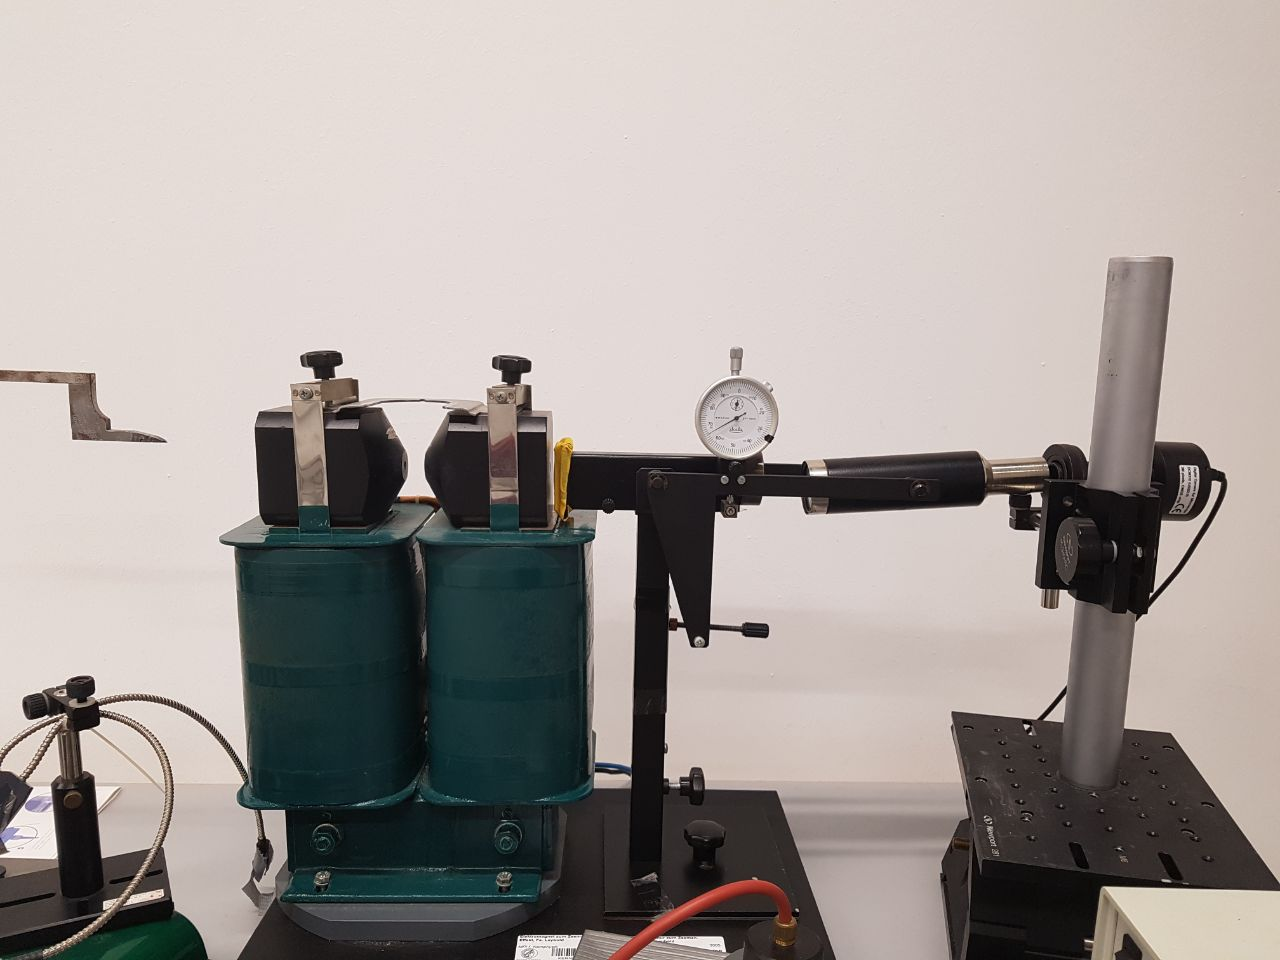
\includegraphics[width=0.6\linewidth]{img/IMG-20180102-WA0000.jpg}
                \caption{Versuchsaufbau, 1. Versuchsteil}
            \end{figure}
        \end{myframe}


    \subsection{2. Versuchsteil - Wellenlängenbestimmung}
        \begin{myframe}{\subsecname}
            \begin{itemize}
                \item Verwendung des Czerny - Turner Spektrometer um das Spektrum aufzunehmen
                \item Kalibrierung des Spektrometers mit Hilfe eines Referenzspektrums
                \item Bestimmung der Wellenlänge der roten Cadmium - Linie und einer unbekannten Linie
            \end{itemize}
        \end{myframe}

        \begin{myframe}{\subsecname}
            \begin{columns}
                \begin{column}{0.48\textwidth}
                    \begin{figure}
                        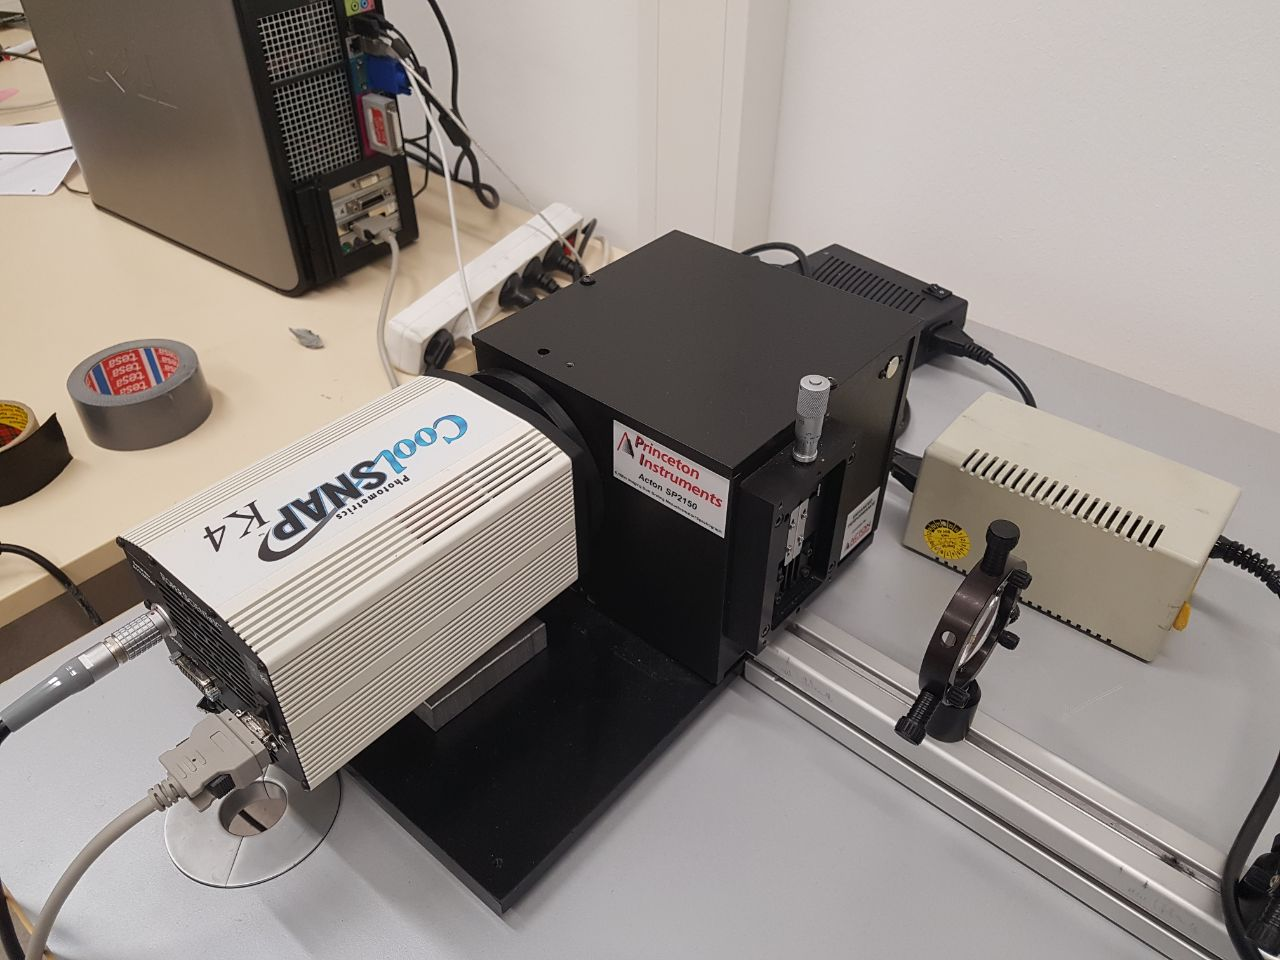
\includegraphics[width=0.8\linewidth]{img/IMG-20180102-WA0002.jpg}
                        \caption{Czerny - Turner Spektrometer}
                    \end{figure}
                \end{column}
                \begin{column}{0.48\textwidth}
                    \begin{figure}
                        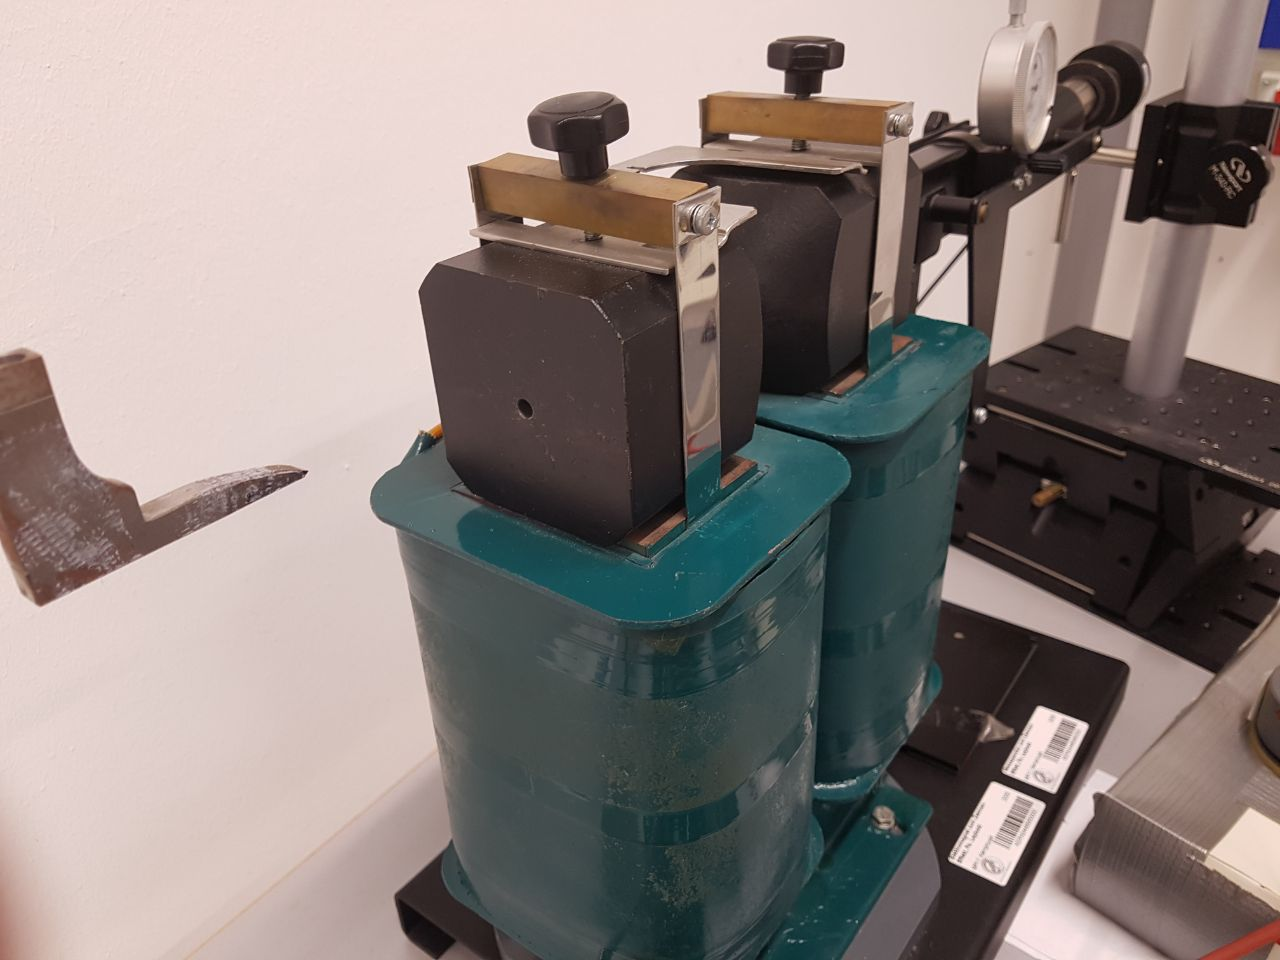
\includegraphics[width=0.8\linewidth]{img/IMG-20180102-WA0003.jpg}
                        \caption{Versuchsaufbau, 2. Versuchsteil}
                    \end{figure}
                \end{column}
            \end{columns}
        \end{myframe}


  % !TeX root = ../pres.tex

\section{Bohr'sches Magneton}
  \subsection{Hysterese Effekt}
    \begin{myframe}{\subsecname}
      \begin{itemize}
        \item Magnetfeldmessung bei 6 Stromstärken zwischen 8 und 13A
        \item für fallende und steigende Stromstärke
        \item Ermittlung des Zusammenhangs zwischen Stromstärke und Magnetfeld
      \end{itemize}

      Resultat:
      \begin{align}
        m_u = \inclineUp\\
        m_d = \inclineDown
      \end{align}

      $\Rightarrow$ Abweichung: < 1$\sigma$
    \end{myframe}

    \begin{myframe}{}
        \begin{figure}
          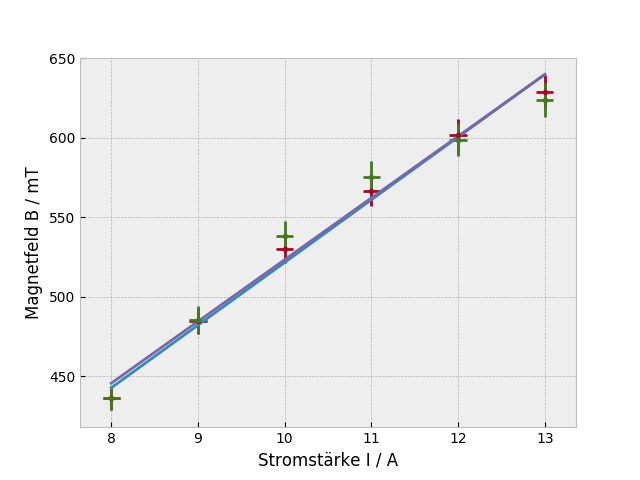
\includegraphics[height=.85\paperheight]{img/hysteresis.png}
          \caption{Hysterese}
          \label{Hysterese}
        \end{figure}
    \end{myframe}

  \subsection{Polarisation}
    \subsubsection{longitudinal}
      \begin{myframe}{\subsecname\ - \subsubsecname}
        \onslide<1,3>{%
          \begin{itemize}
            \item mit und ohne linearem Polarisationsfilter: 2 Linien pro Beugungsordnung
            \item[$\rightarrow$] zirkulär polarisiert
            \item[]
            \item<3> mit $\lambda /4$-Filter in linear polarisiertes umwandeln
            \item<3> jetzt erhält man eine Linie pro Beugungsordnung, nach linearem Polarisationsfilter
            \item[$\rightarrow$]<3> Rotation des Linearfilters um 90° wechselt zwischen beiden Linien
          \end{itemize}
        }
        \onslide<2,4>{%
          \vspace{-.35\paperheight}
        }
        \begin{figure}
          \centering
          \onslide<2>{%
            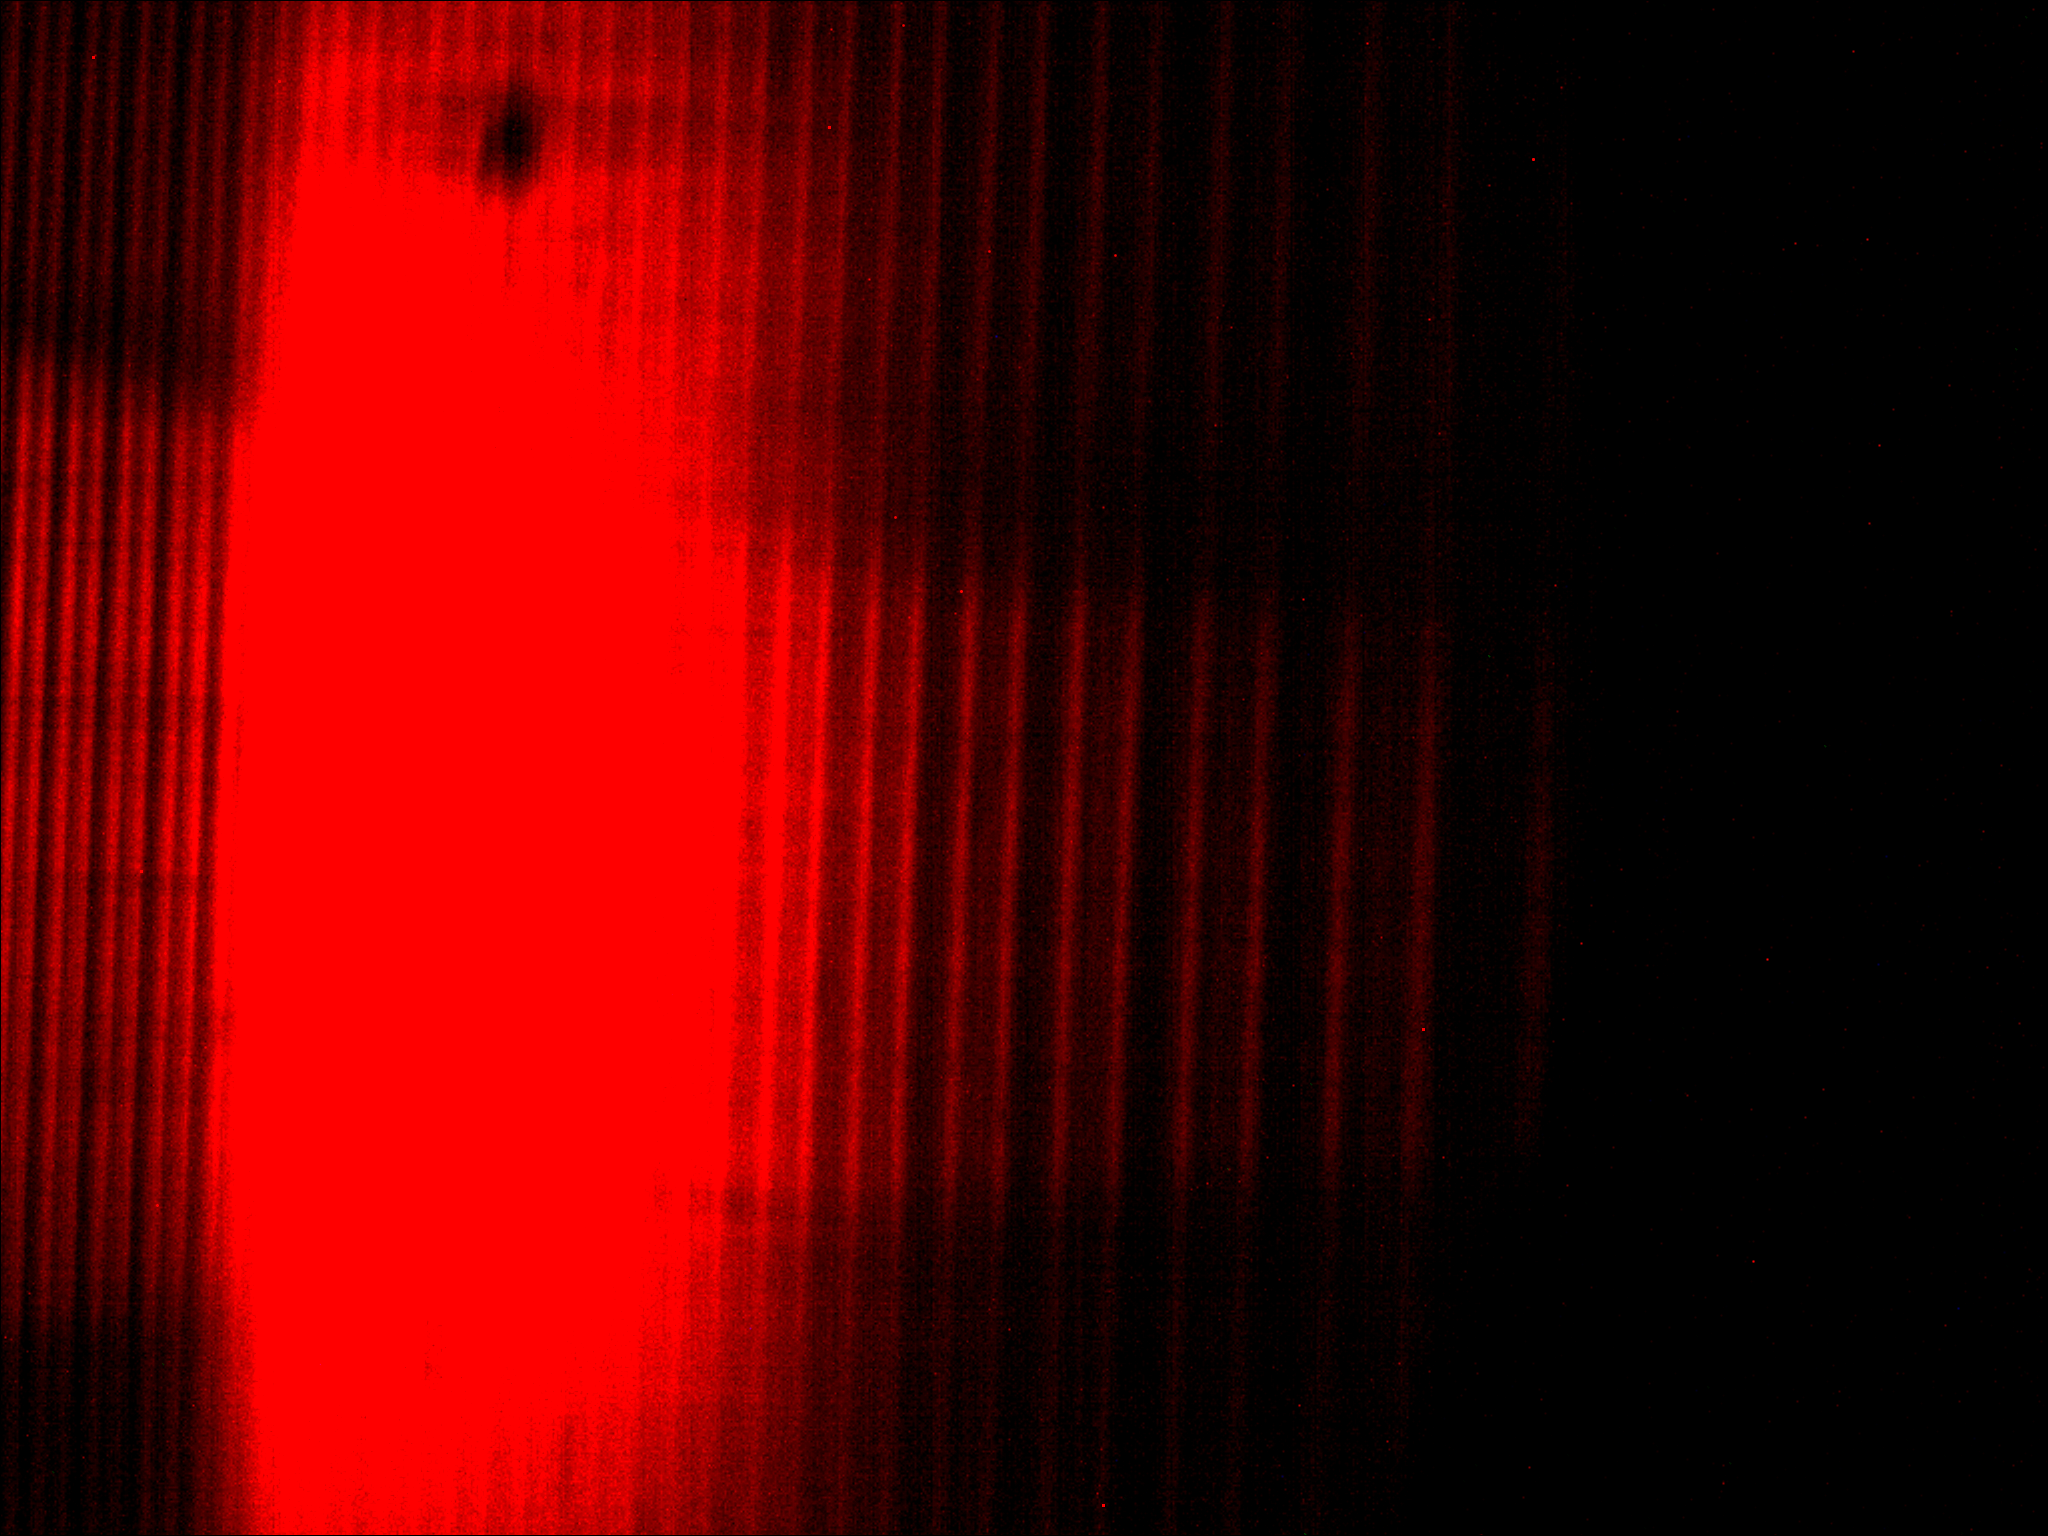
\includegraphics[height=.6\paperheight]{img/long_ohne.png}
            \caption{longitudinale Polarisation ohne Fiter}
            \label{long_ohne}
          }
          \onslide<4>{%
            \vspace{-.75\paperheight}
            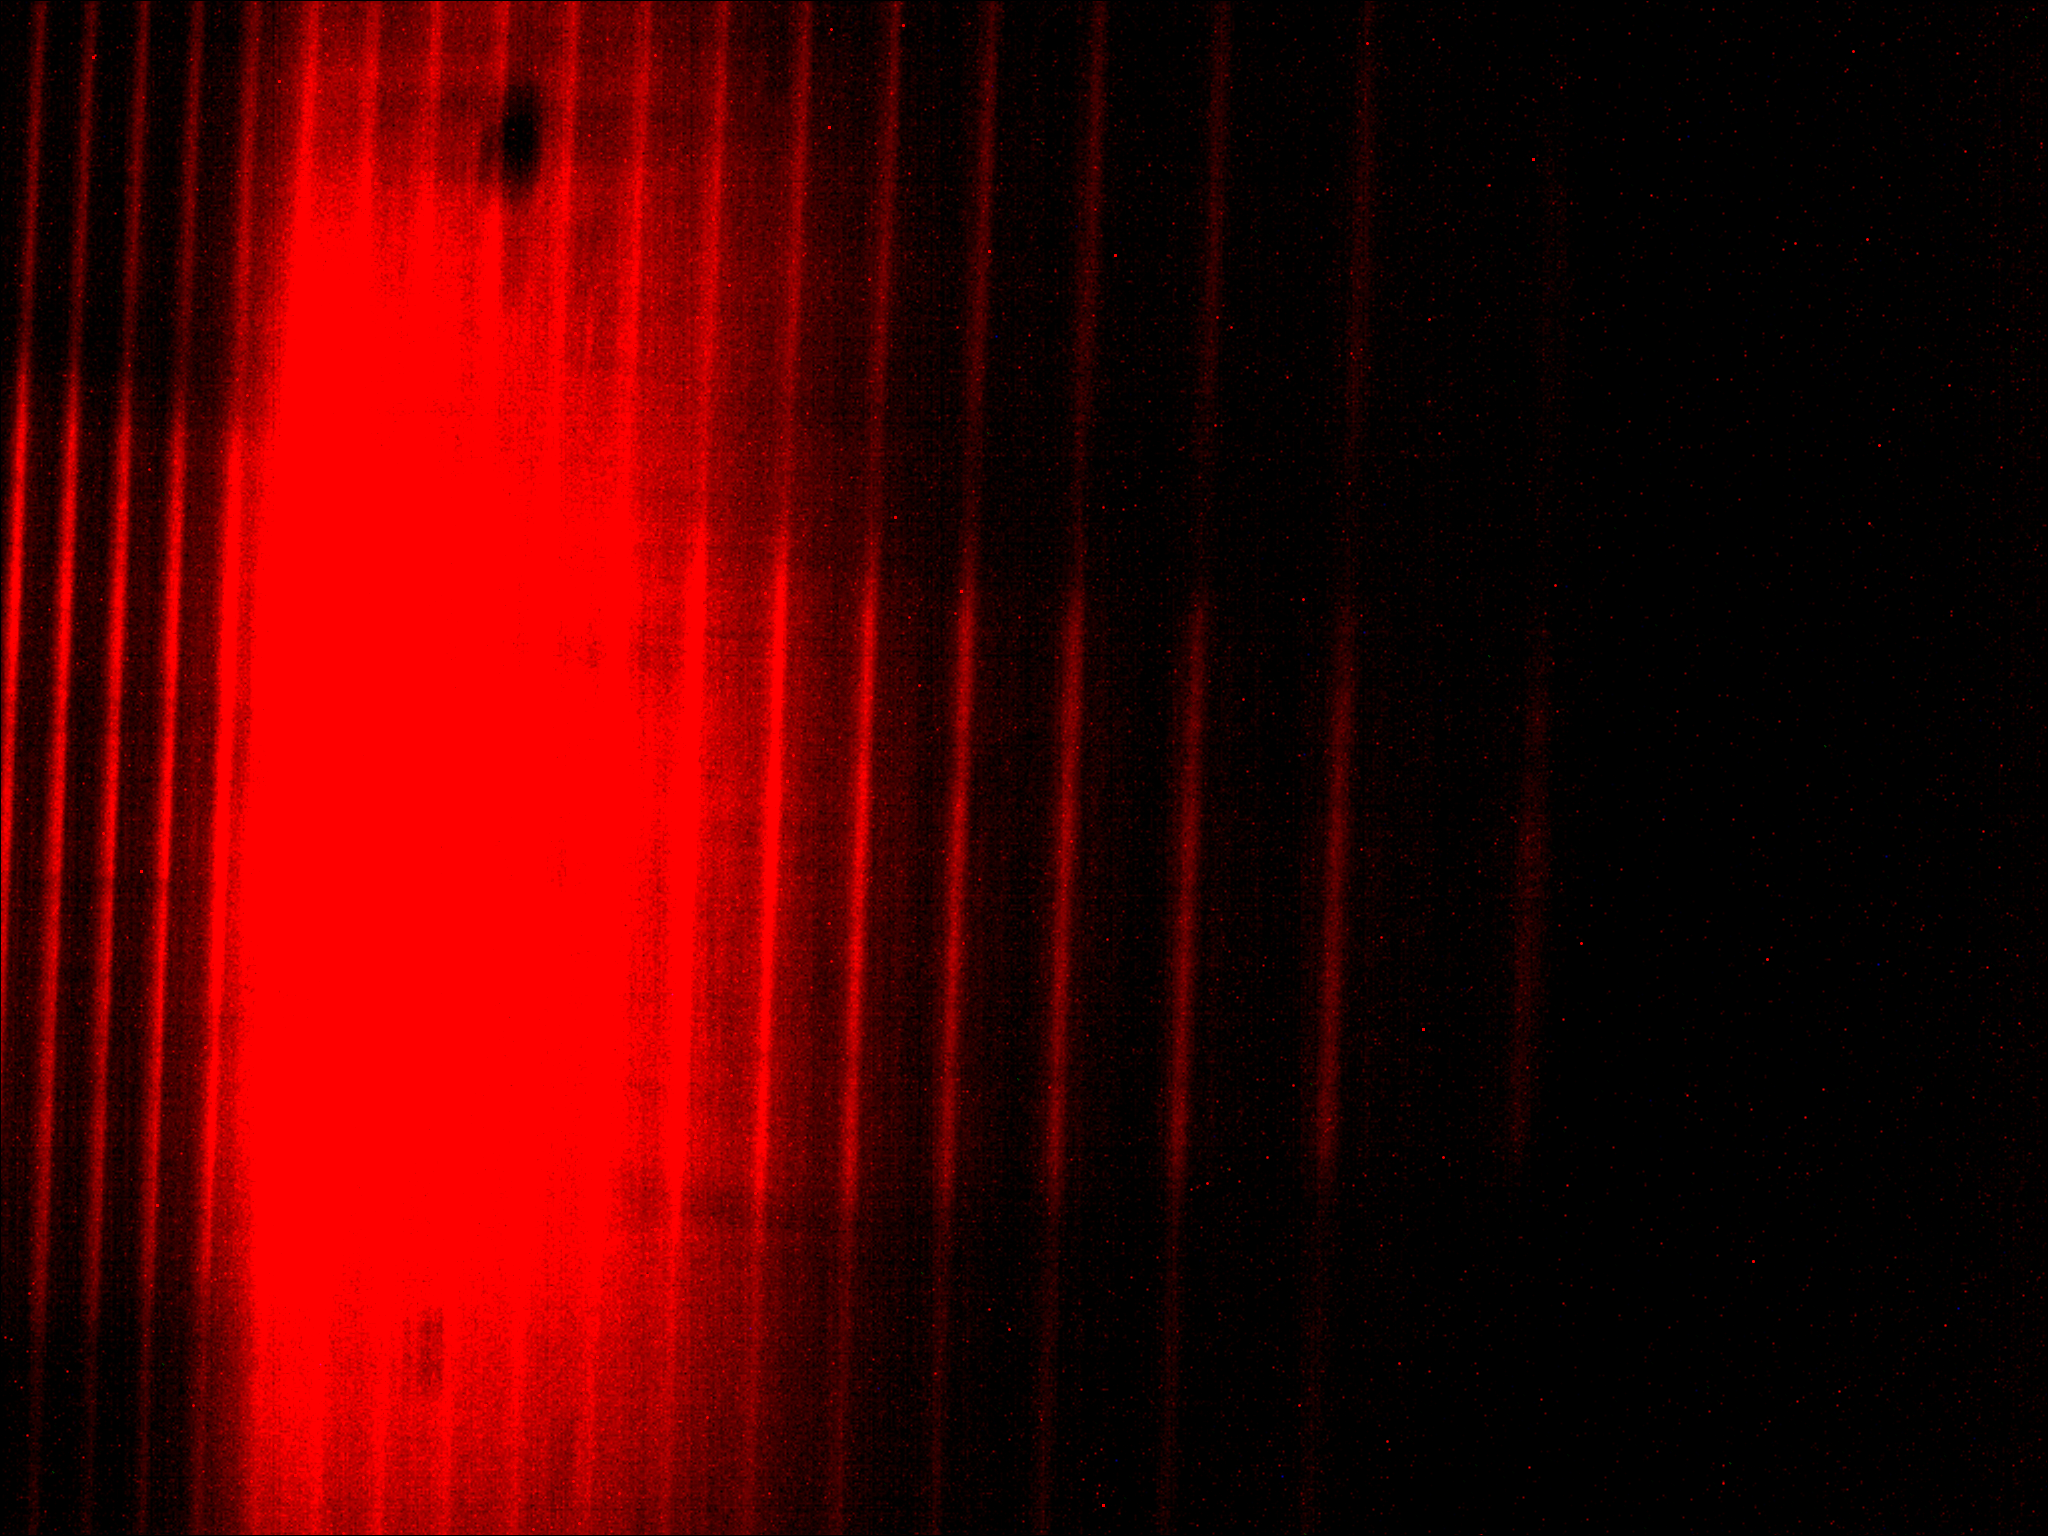
\includegraphics[width=.5\paperwidth, trim={0 650pt 0 200pt}, clip]{img/long_2}
            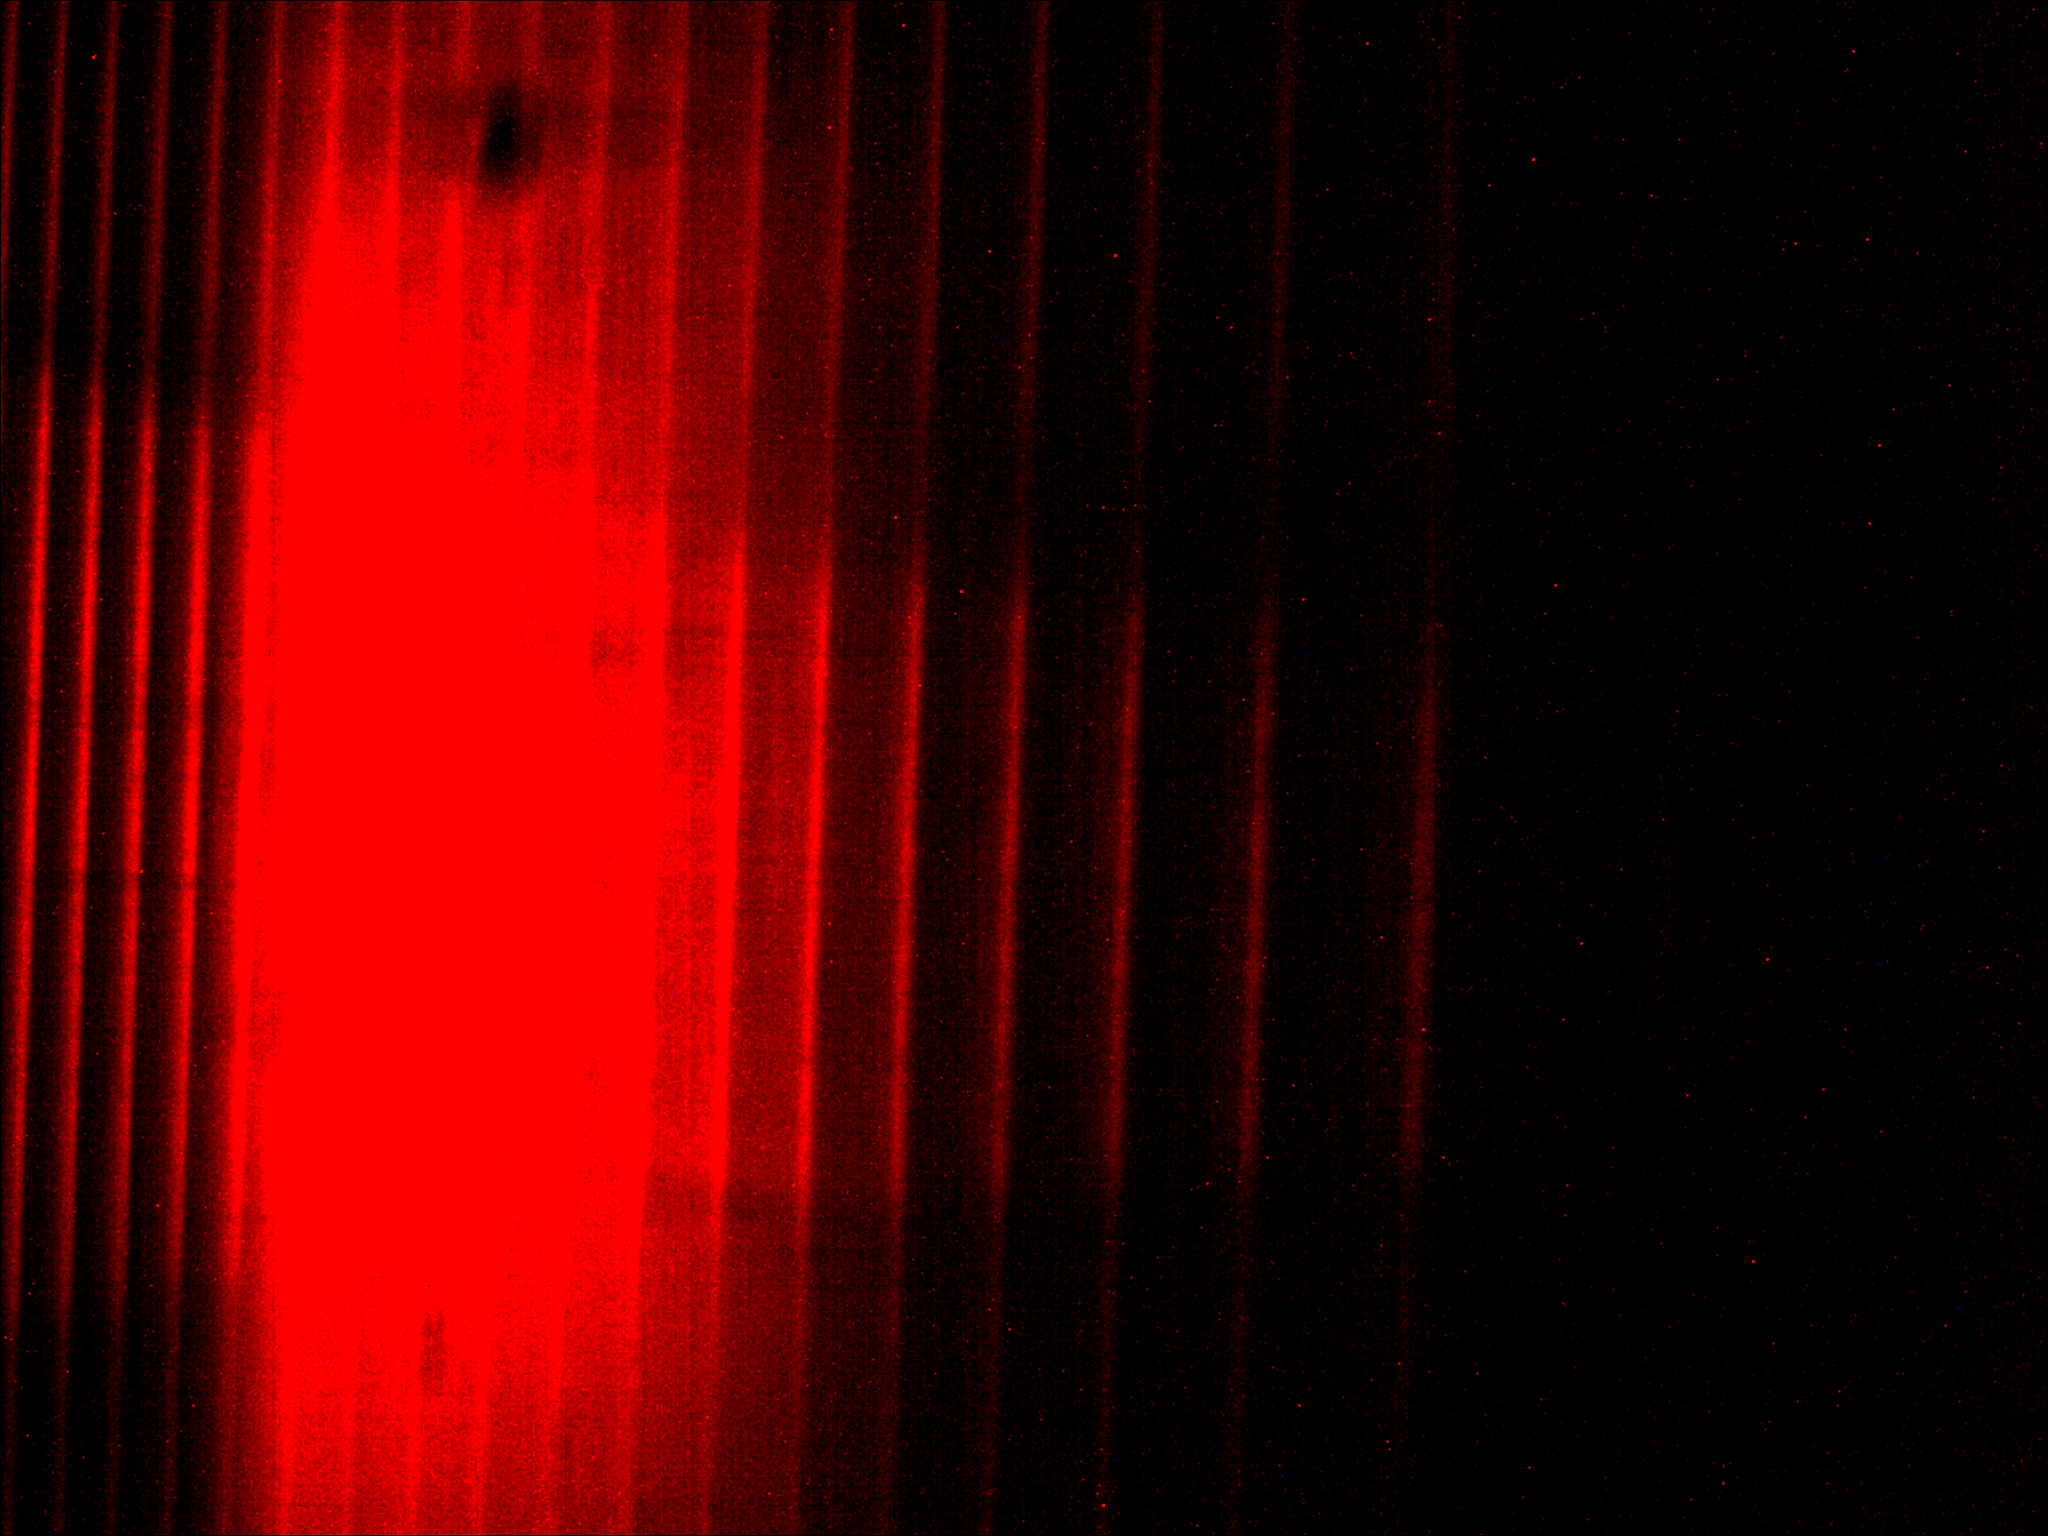
\includegraphics[width=.5\paperwidth, trim={0 0 0 886pt}, clip]{img/long_1}
            \caption{Beobachtete Linien in longitudinaler Richtung, mit $\lambda$/4-Filter und linearem Polarisationsfilter}
            \label{long_mit}
          }
        \end{figure}
      \end{myframe}

      \subsubsection{transversal}
        \begin{myframe}{\subsecname\ - \subsubsecname}
           \begin{itemize}
             \item Beobachtung von 3 Linien
             \item[$\rightarrow$] Rotation des Linearfilters um 90° wechselt zwischen den $\sigma$-Linien und der $\pi$-Linie
             \item[$\rightarrow$] linear polarisiert
           \end{itemize}
        \end{myframe}

        \begin{myframe}{\subsecname\ - \subsubsecname}
          \begin{figure}
            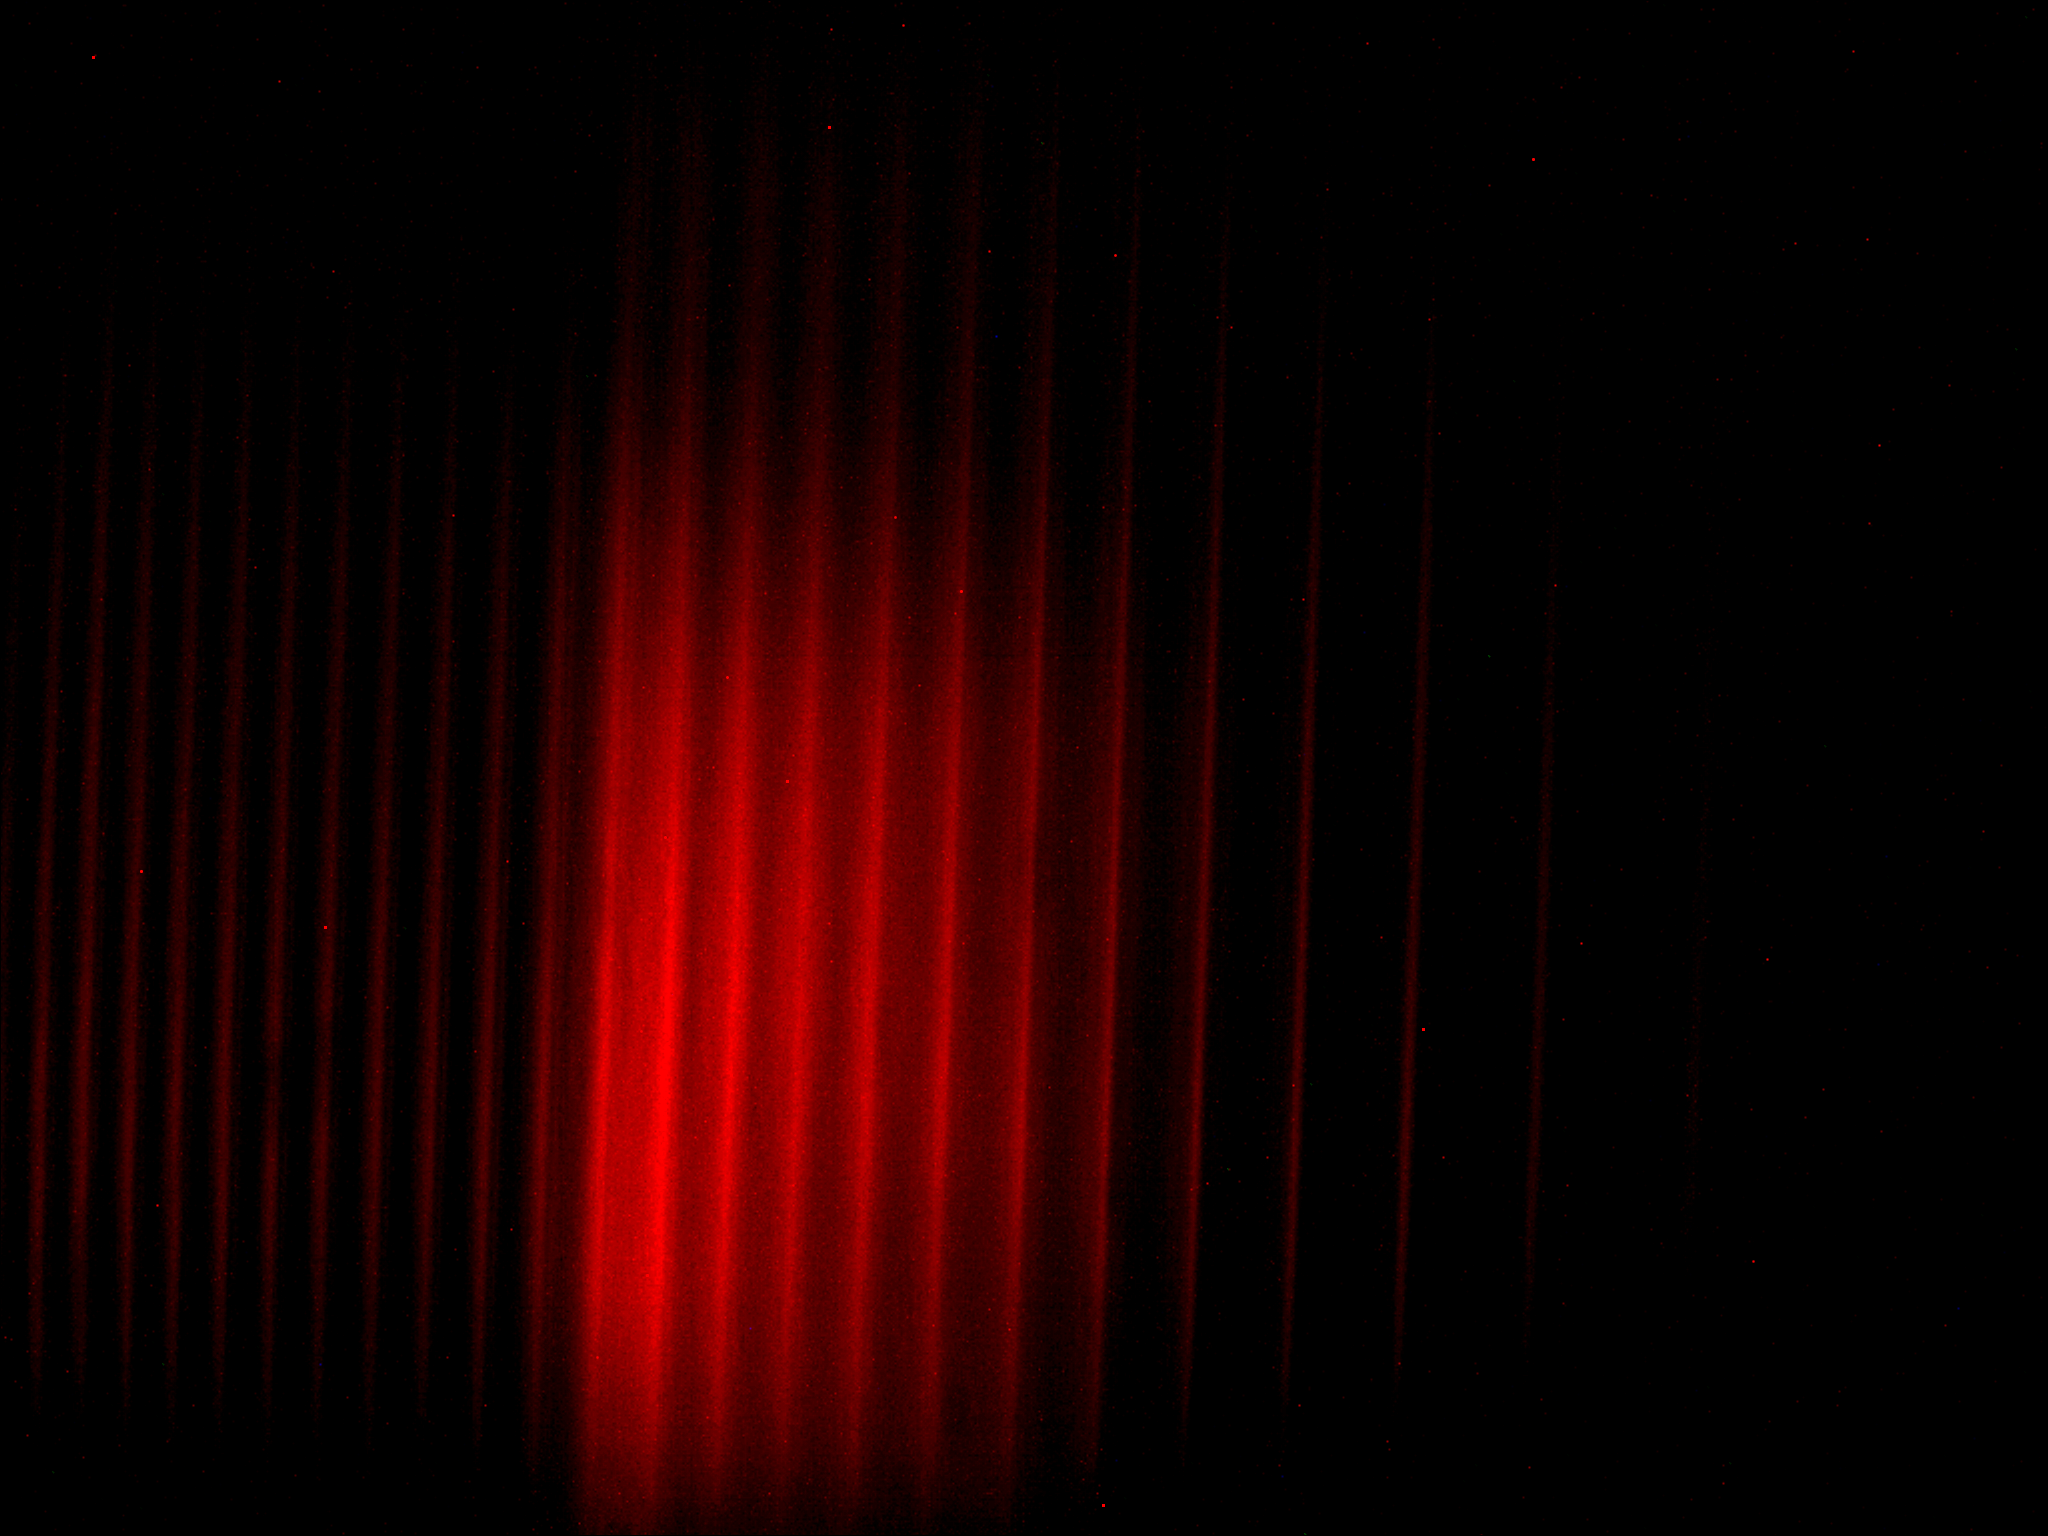
\includegraphics[width=.8\paperwidth, trim={0 300pt 0 900pt}, clip]{img/trans_pi}
            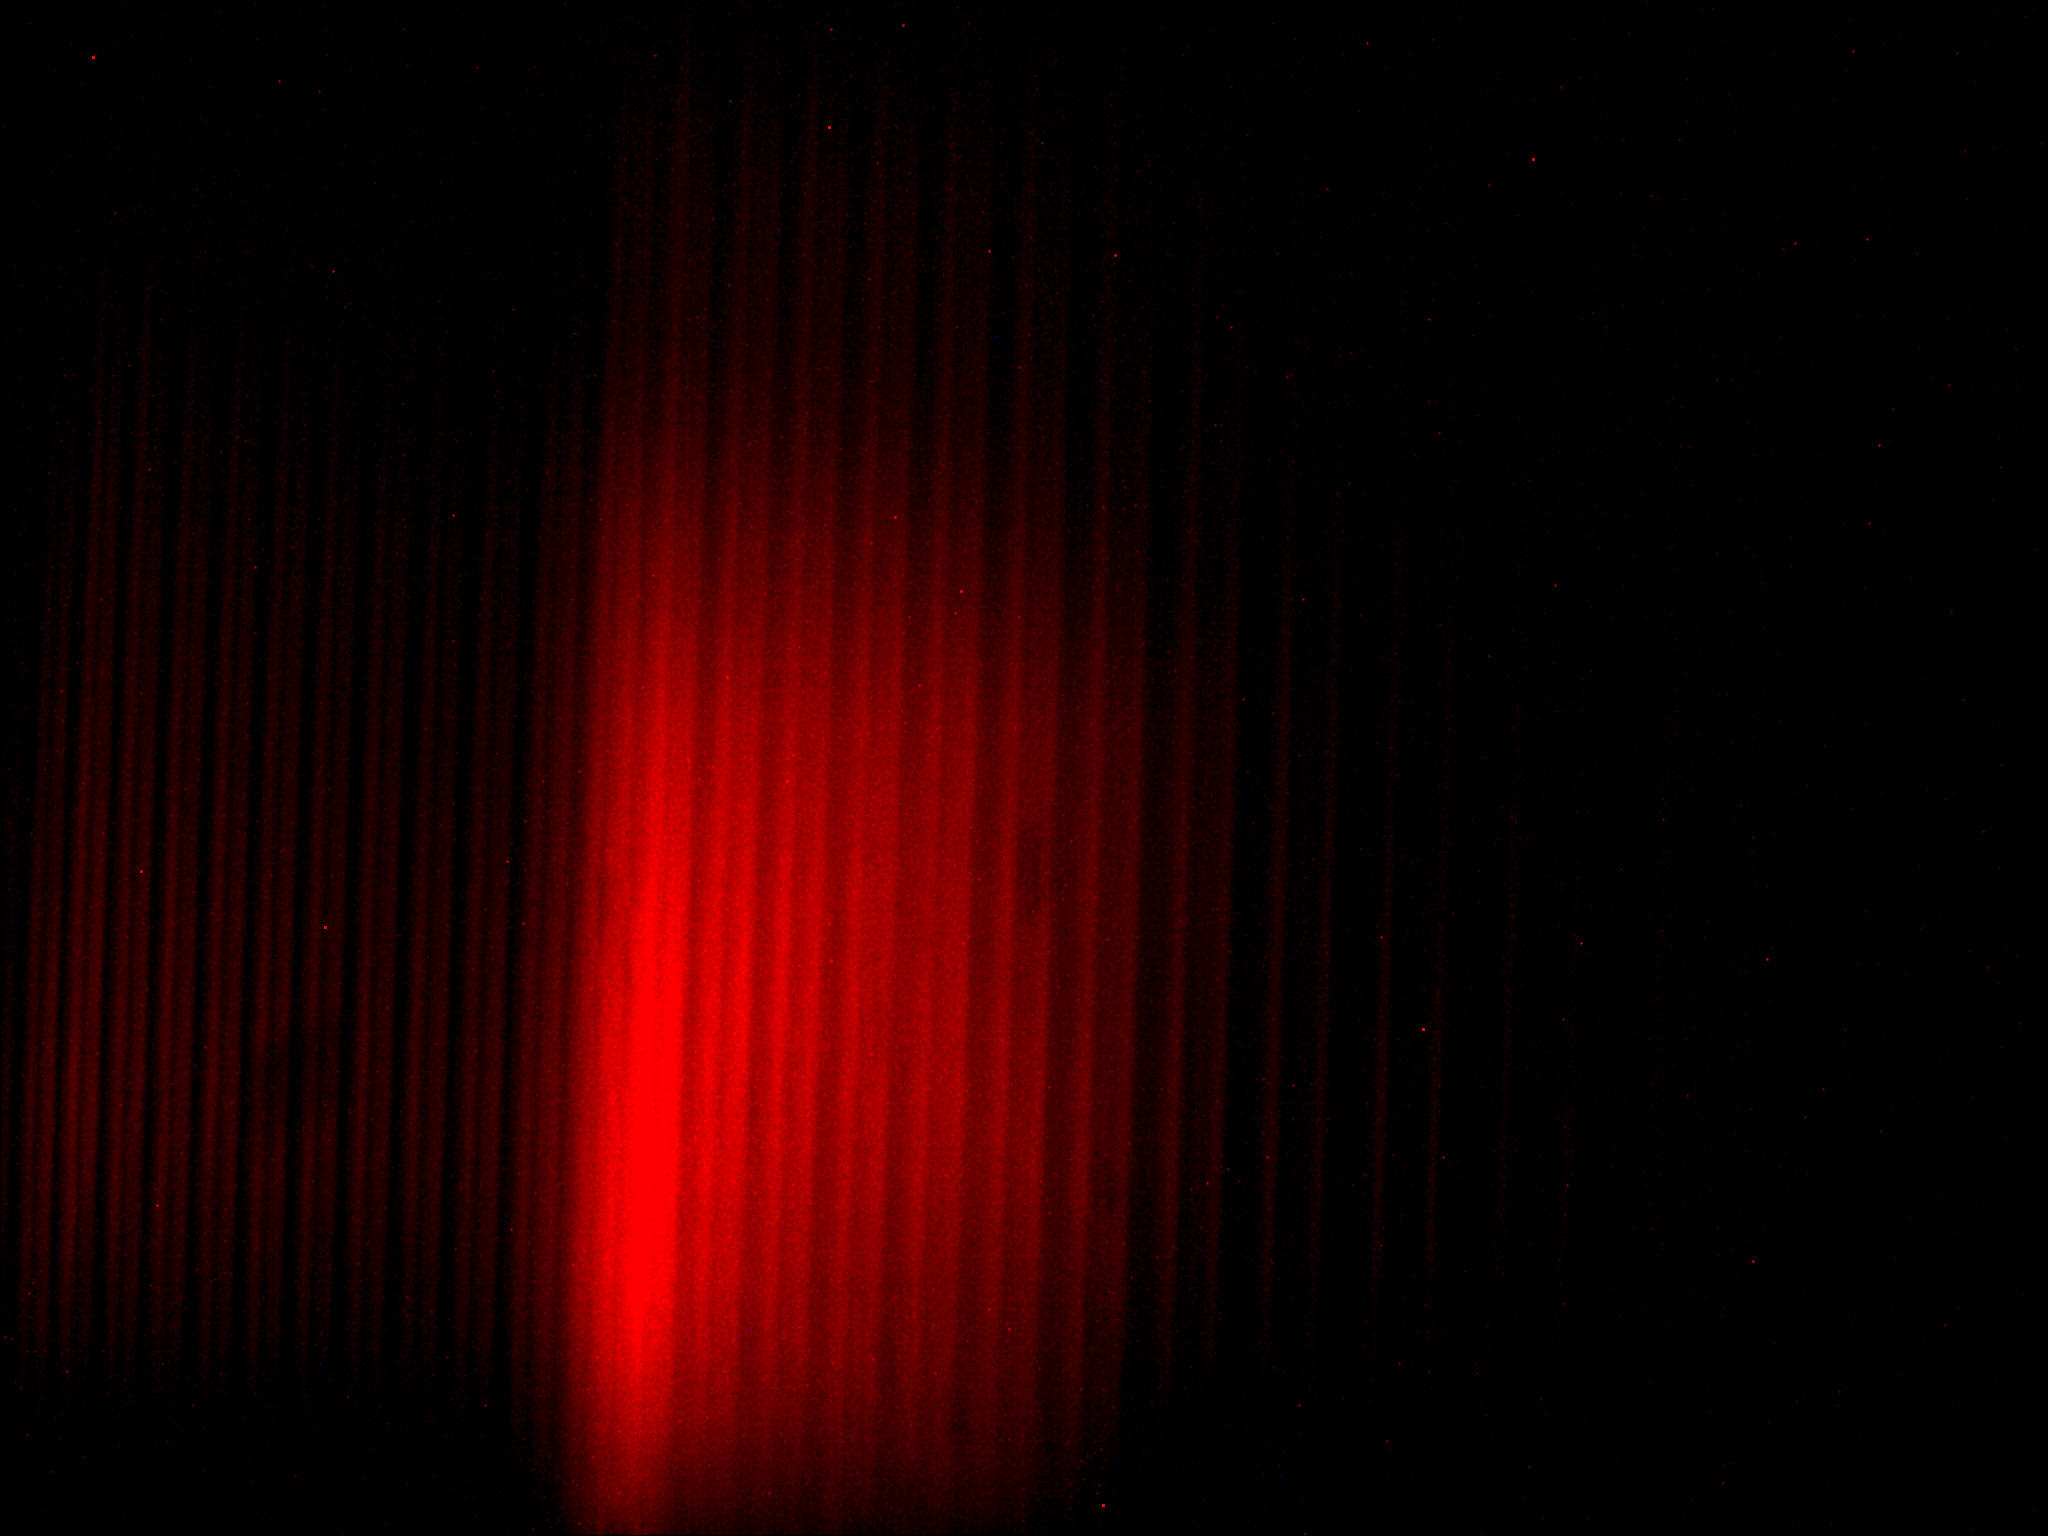
\includegraphics[width=.8\paperwidth, trim={0 300pt 0 900pt}, clip]{img/trans_sig}
            \caption{Beobachtete Linien in transversaler Ausrichtung, mit linearem Polarisationsfilter}
            \label{trans}
          \end{figure}
        \end{myframe}

  \subsection{Bestimmung der Wellenlängenverschiebung}
    \subsubsection{Positionsbestimmung}
      \begin{myframe}{\subsecname\ - \subsubsecname}
        \begin{itemize}
            \item Bestimmung der px-Position von $\sigma$- und $\pi$-Linien
            \item 5 Ordungen
            \item Fit der Peaks für Position und Fehler
        \end{itemize}
      \end{myframe}
      \begin{myframe}{}
          \begin{figure}
              \centering
              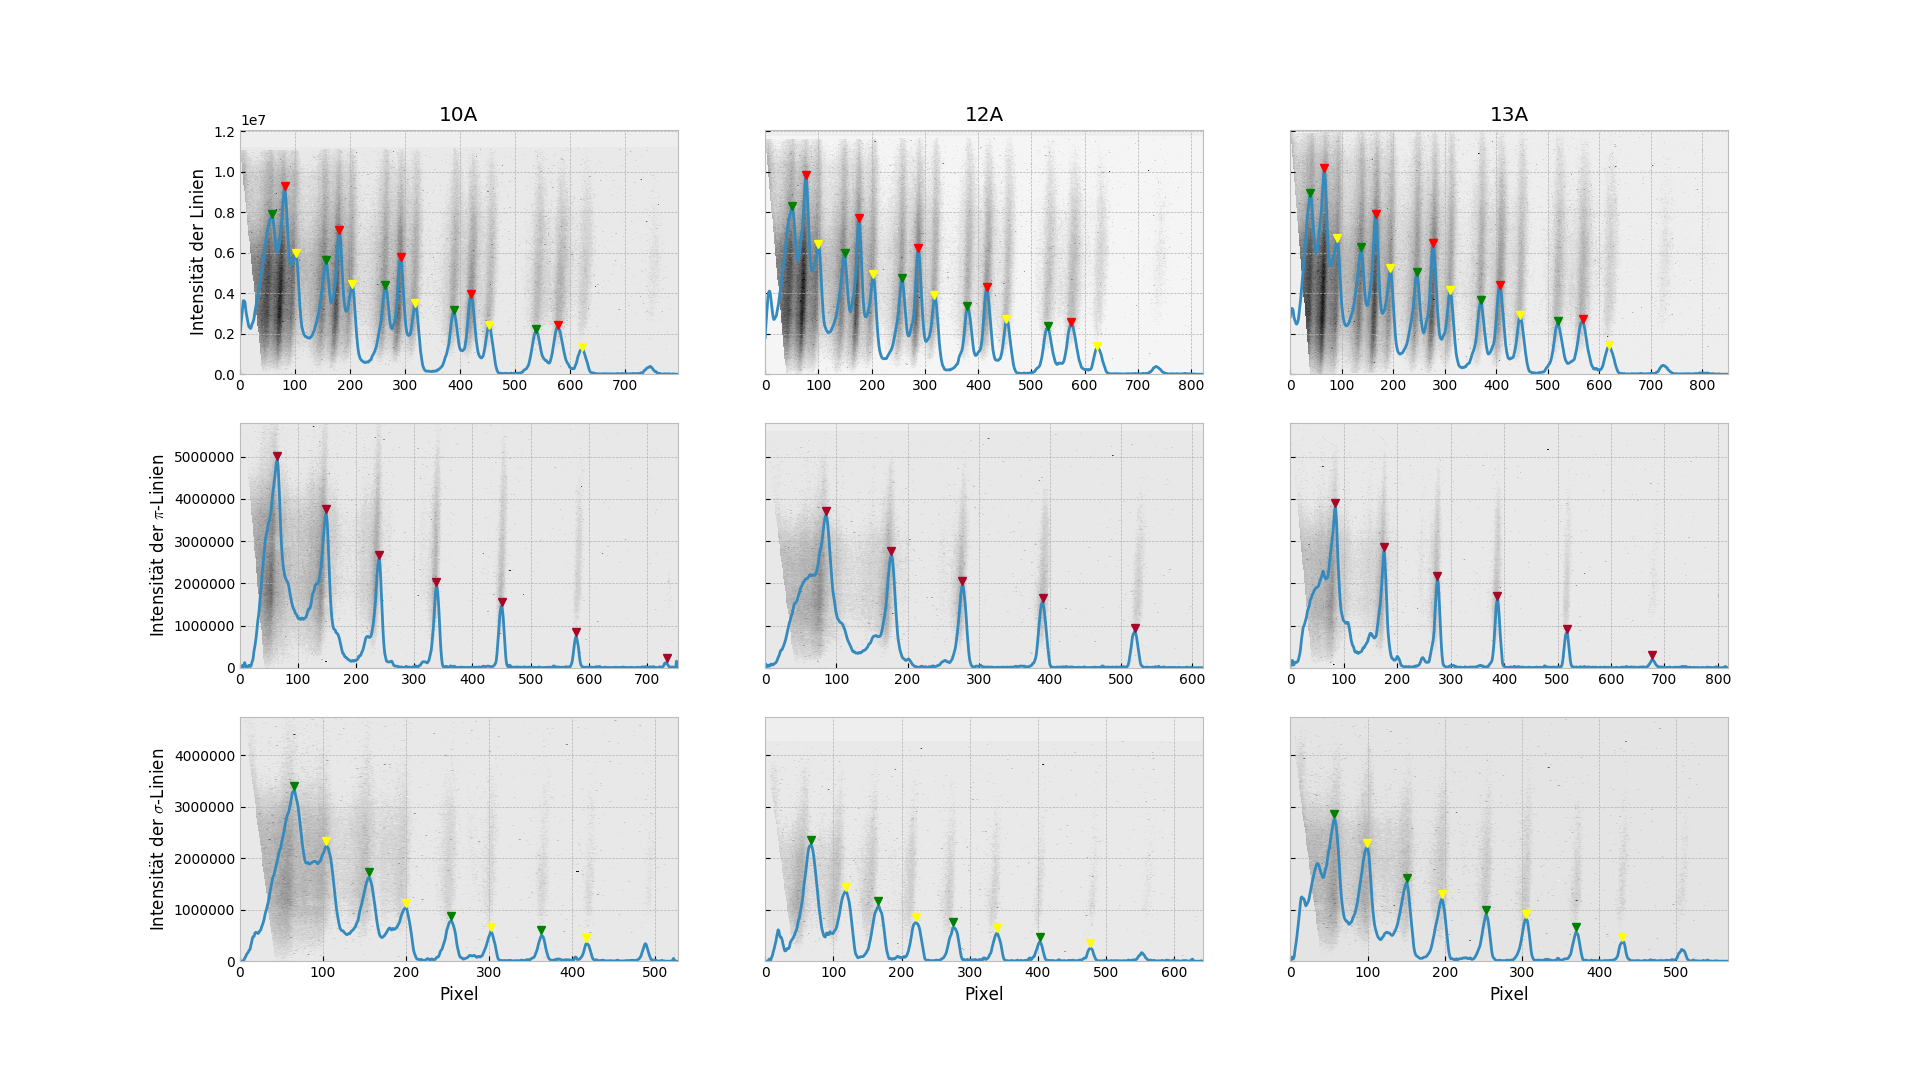
\includegraphics[width=.85\paperwidth]{img/peaks.png}
              \caption{Gefittete Positionen der Peaks}
          \end{figure}
      \end{myframe}

    \subsubsection{Ordnungsverschiebung}
      \begin{myframe}{\subsecname\ - \subsubsecname}
        Zuordung
        \begin{tabular}{p{0.48\textwidth}p{0.4\textwidth}}
          \begin{itemize}
            \item (theoretische) ganzzahligen Ordnung
            \item kontinuierliche Polynomfitfkt
          \end{itemize} &
          \begin{itemize}
            \item[] $\mapsto \pi$-linien
            \item[] $\mapsto \sigma$-Linien
          \end{itemize} \\
        \end{tabular}
        $\Rightarrow$ beobachtete Verschiebung der Beugungsordnung zwischen drei Peaks
      \end{myframe}
      
      \begin{myframe}{}
          \begin{figure}
              \centering
              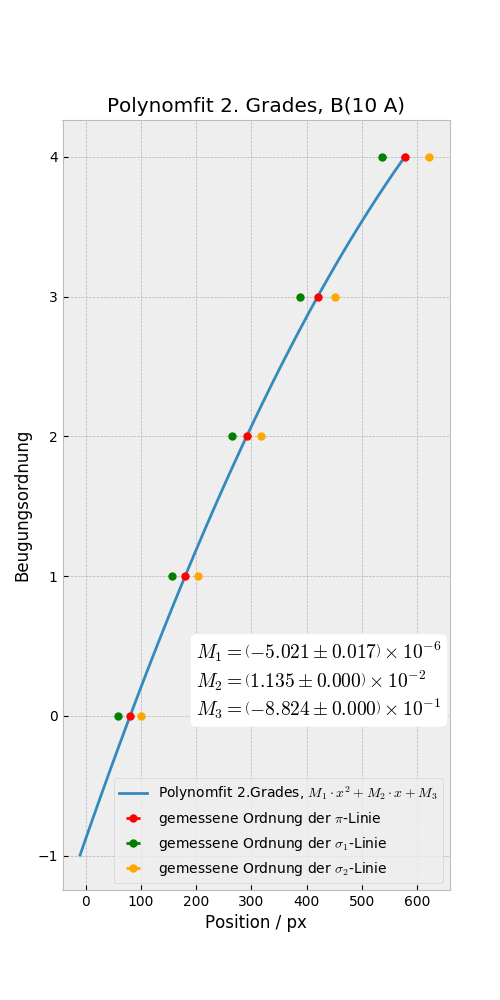
\includegraphics[height=.85\paperheight]{img/sco_10A}
              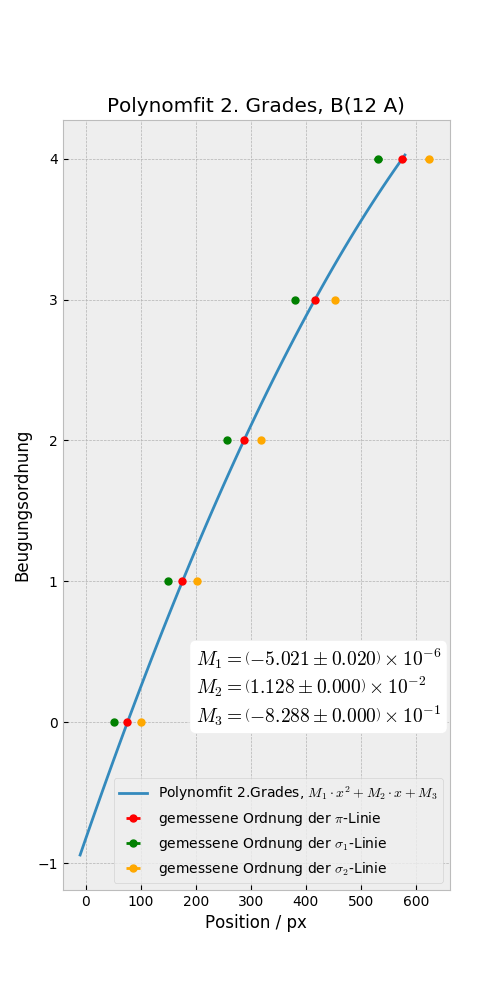
\includegraphics[height=.85\paperheight]{img/sco_12A}
              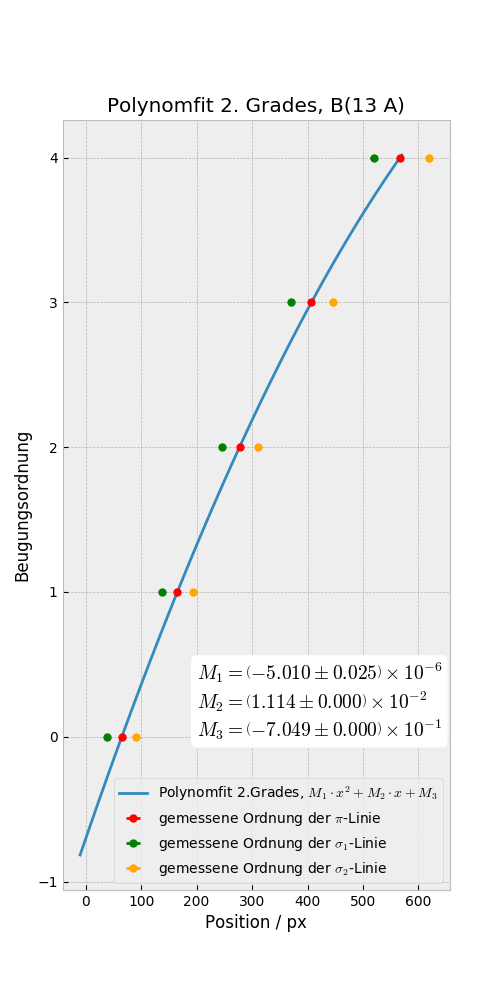
\includegraphics[height=.85\paperheight]{img/sco_13A}
              \caption{Polynomfits für die drei Stromstärken} 
          \end{figure}
      \end{myframe}

    \subsubsection{Wellenlängenverschiebung}
      \begin{myframe}{\subsecname\ - \subsubsecname}
        für kleine Verschiebungen gilt:
        \begin{align}
          \delta\lambda = \frac{\delta a}{\Delta a}\cdot \Delta\lambda\approx\delta k\cdot\lambda k,
          &\qquad\Delta\lambda = \frac{\lambda^2}{2d\cdot\sqrt{n^2-1}}\\
        \end{align}
        \scriptsize (n = \SI{1.4567}{}, d=\SI{4.04e-3}{m})
      \end{myframe}
      \begin{myframe}{}
          \begin{figure}
              \centering
              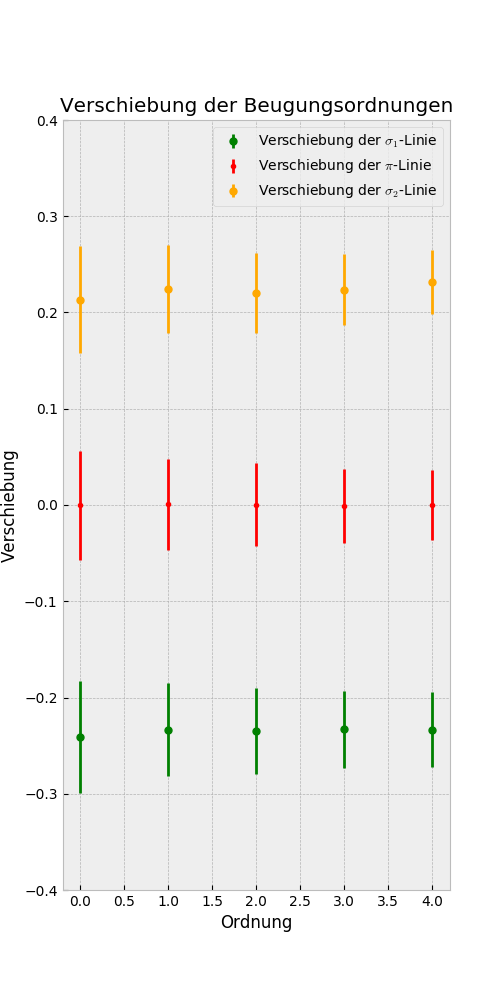
\includegraphics[height=.85\paperheight]{img/diff_sco10A}
              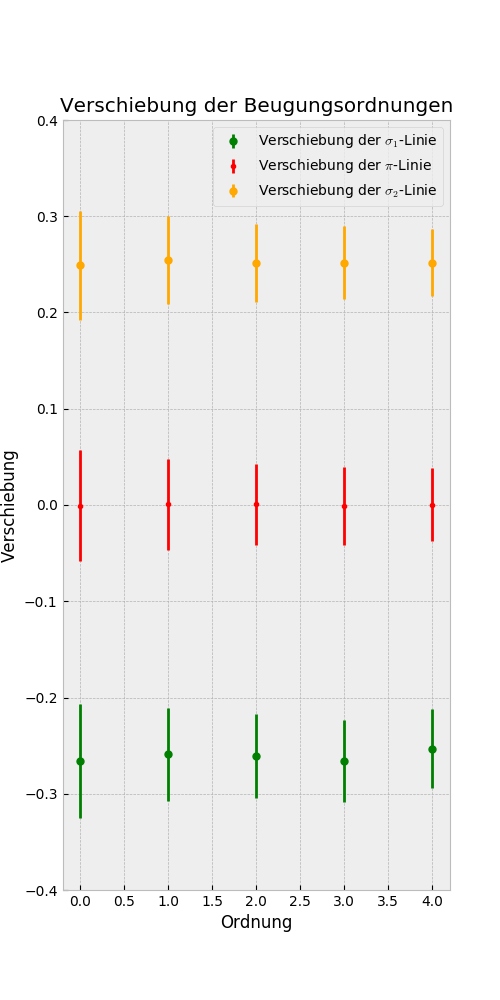
\includegraphics[height=.85\paperheight]{img/diff_sco12A}
              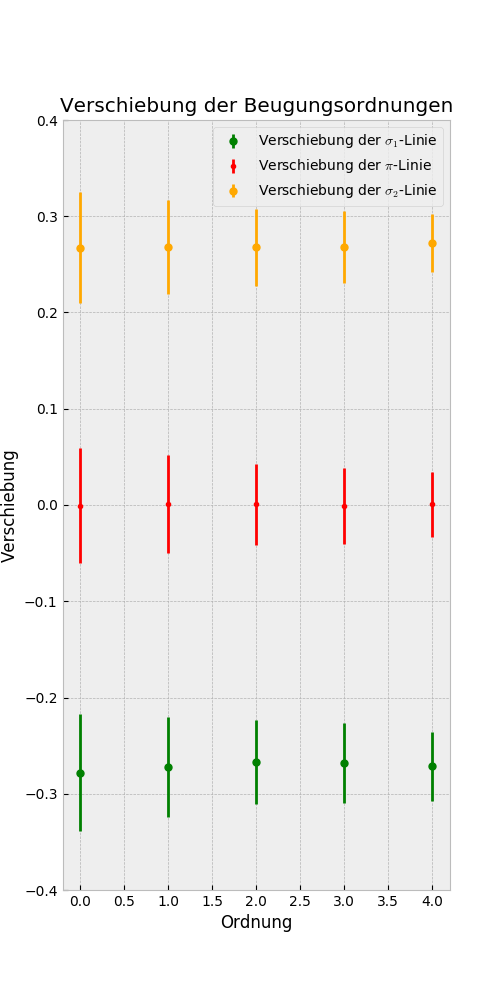
\includegraphics[height=.85\paperheight]{img/diff_sco13A}
              \caption{Verschiebung der Beugungsordnung} 
          \end{figure}
      \end{myframe}
      \begin{myframe}{\subsecname\ - \subsubsecname}
          mit der von uns sp\"ater bestimmten Wellenl\"ange von Cadmium
          \begin{align}
              \lambda_{Cd}=\lambdaCd 
          \end{align} 
          ergeben sich folgende Wellenl\"angenverschiebungen
          \begin{table}[H]
              \centering
              \begin{tabular}{lll}
\toprule
I/A & $\delta\lambda_1/\si{pm}$ & $\delta\lambda_2/\si{pm}$ \\
\midrule
 10 &       $-11.394 \pm 0.140$ &        $10.788 \pm 0.294$ \\
 12 &       $-12.656 \pm 0.239$ &        $12.197 \pm 0.087$ \\
 13 &       $-13.153 \pm 0.187$ &        $13.019 \pm 0.093$ \\
\bottomrule
\end{tabular}

              \caption{$\delta\lambda$ für die drei beobachteten Stromstärken, sowie für beide $\sigma$-Linien}
          \end{table}
      \end{myframe}
  \subsection{Bestimmung des Bohr'schen Magneton}
  \subsubsection{Methode 1: statistisches Mittel}
      \begin{myframe}{\subsecname\ - \\\subsubsecname}
         \begin{table}[H]                                                             
             \centering                                                               
             \begin{tabular}{lll}
\toprule
I/A & $\delta\lambda_1/\si{pm}$ & $\delta\lambda_2/\si{pm}$ \\
\midrule
 10 &       $-11.394 \pm 0.140$ &        $10.788 \pm 0.294$ \\
 12 &       $-12.656 \pm 0.239$ &        $12.197 \pm 0.087$ \\
 13 &       $-13.153 \pm 0.187$ &        $13.019 \pm 0.093$ \\
\bottomrule
\end{tabular}
                                                  
             \caption{$\delta\lambda$ für die drei beobachteten Stromstärken, sowie für beide $\sigma$-Linien}                                                 
         \end{table}
         \begin{align}
             \Rightarrow \quad \mu_B &= \magnetonOne\\
             \mu_{B, theo} &= \magnetonTheo \quad \rightarrow \SI{1.6}{\sigma}
         \end{align}
      \end{myframe}      
  \subsubsection{Methode 2: linearer Fit}
        \begin{myframe}{\subsubsecname}
            \begin{figure}
                \centering
                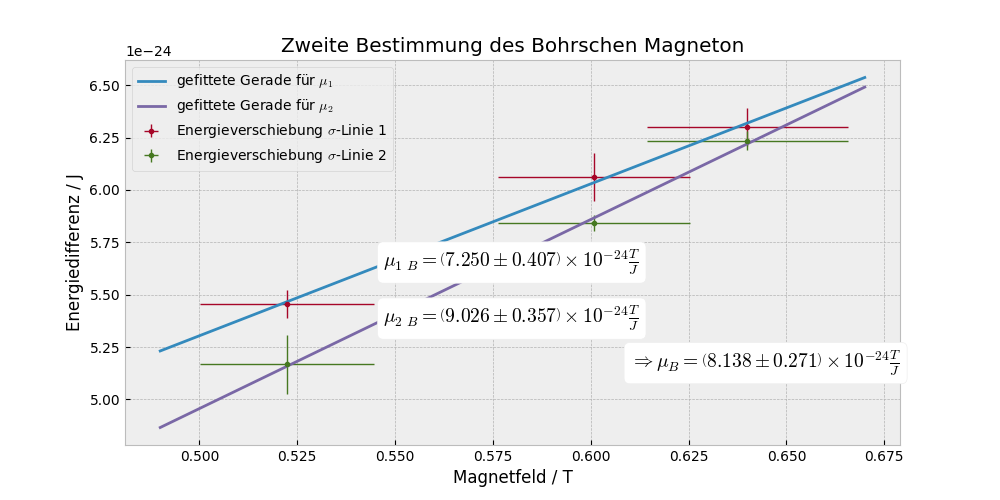
\includegraphics[width=.85\paperwidth]{img/mu_B2}
                \caption{Graphische Bestimmung des Bohr’schen Magneton} 
            \end{figure}            
        \end{myframe}

  % !TeX root = ../pres.tex

\section{Wellenlänge}
    \begin{myframe}{}
        \begin{figure}
            \centering
            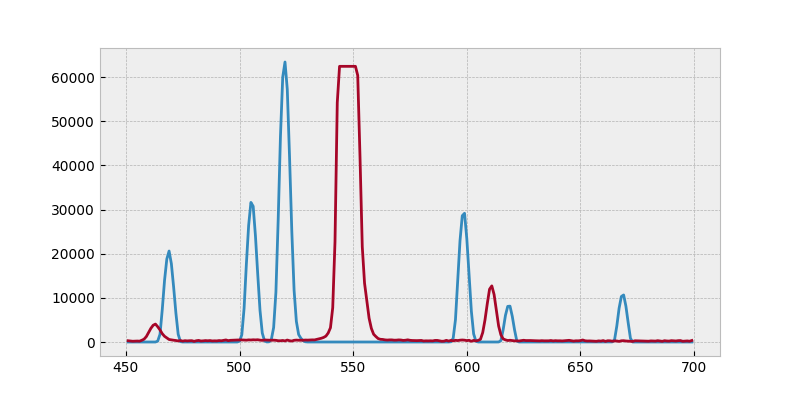
\includegraphics[width=.8\paperwidth]{img/wl.png}
            \caption{Cadmium- (Rot) und Neon- (Blau) Linien (y: Int arbitr\"ar, x: pos in px)}
        \end{figure}
    \end{myframe}

    \begin{myframe}{}
        \begin{figure}
            \centering
            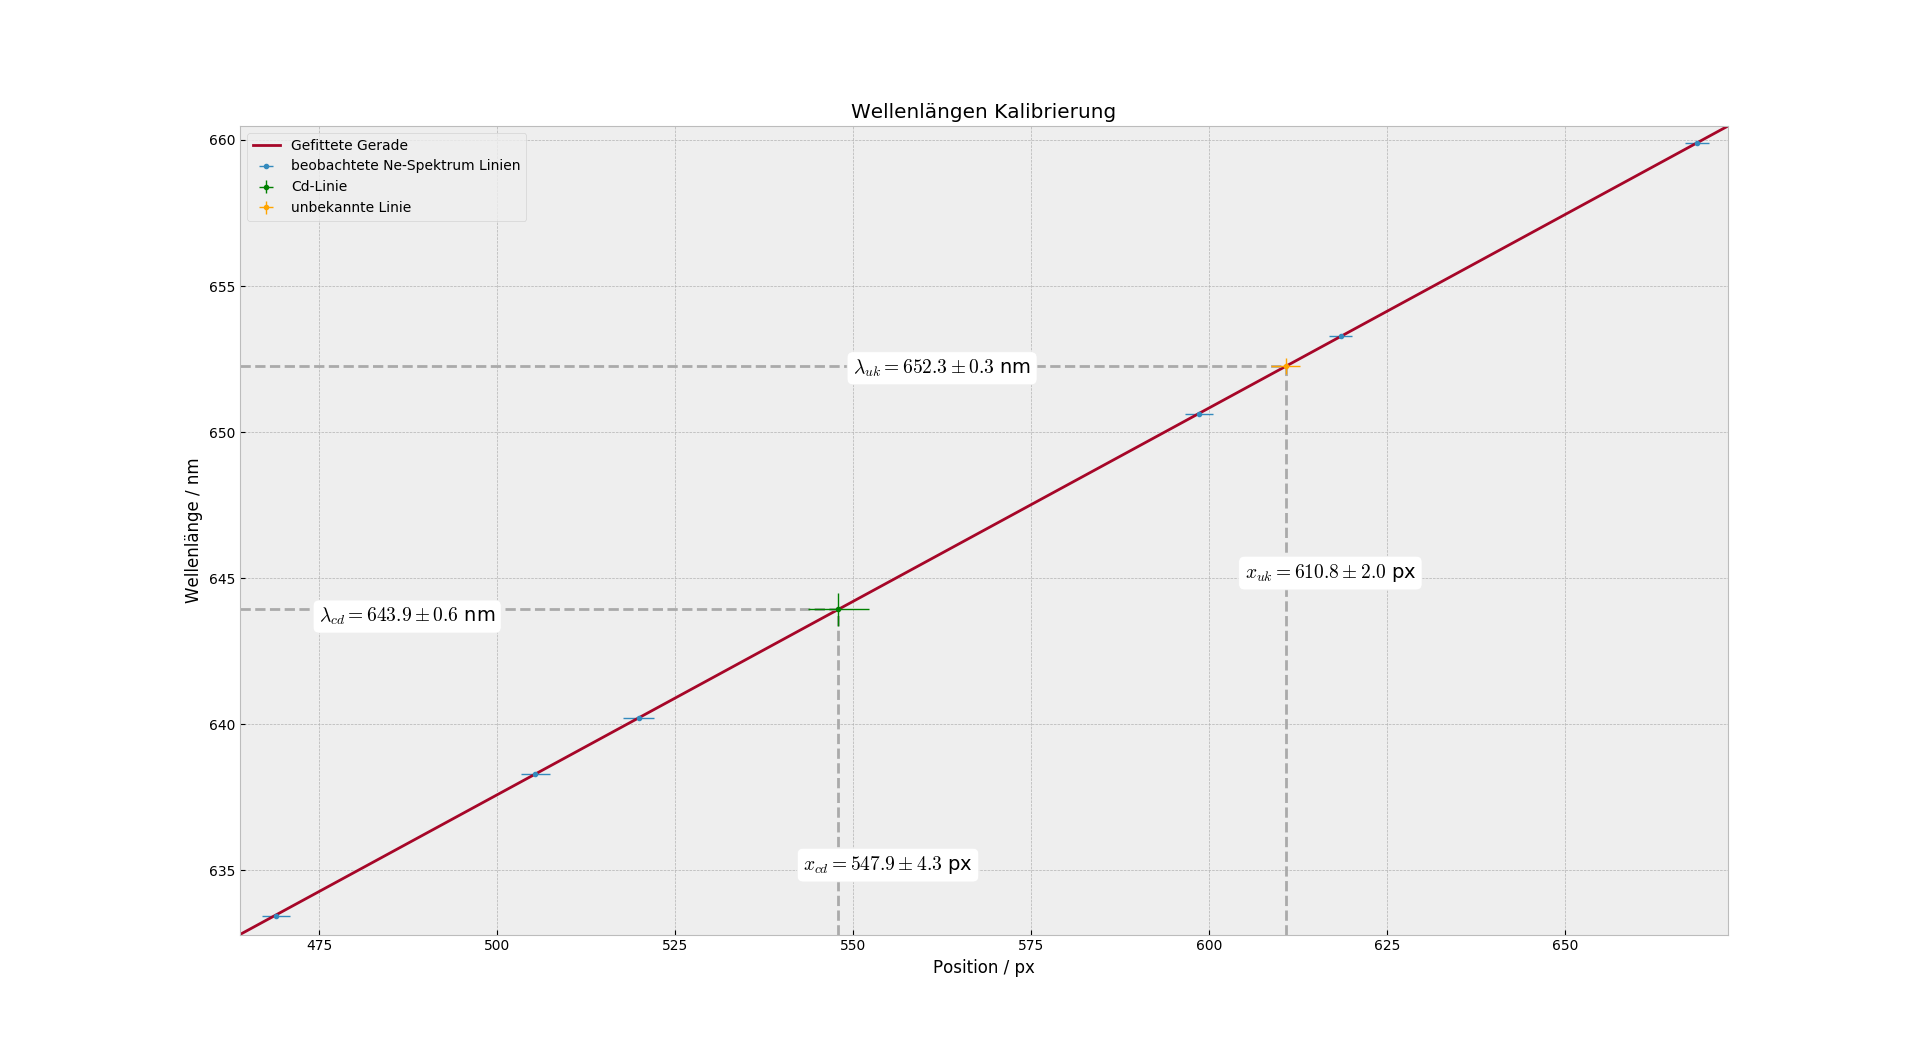
\includegraphics[width=.8\paperwidth]{img/wl_ne_cal}
            \caption{Zusammenhang zwischen Position und Wellenlänge in unseren Beobachtungen}
        \end{figure}
    \end{myframe}

    \subsection{Cadmium-Linie}
        \begin{myframe}{\subsecname}
            \begin{minipage}{.3\textwidth}
                \begin{figure}
                    \centering
                    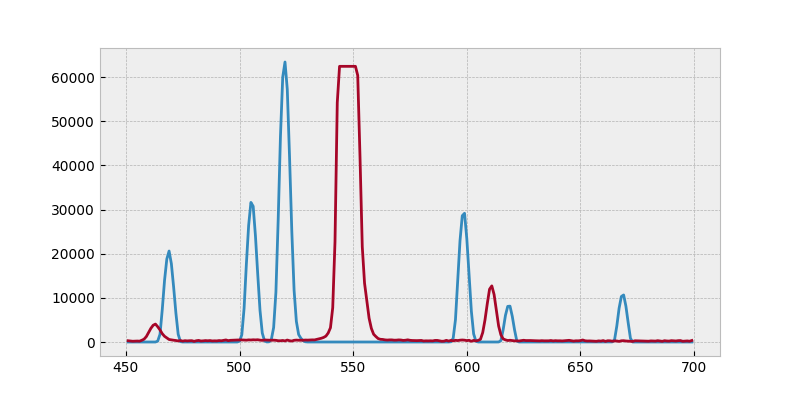
\includegraphics[height=.32\textheight, trim={1.2cm 0 17.5cm 1cm}, clip]{img/wl}
                    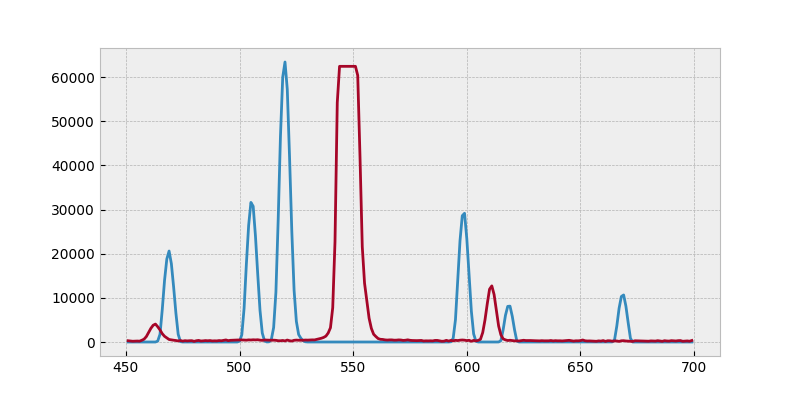
\includegraphics[height=.32\textheight, trim={4cm 0 7cm 1cm}, clip]{img/wl}
                    \caption{Intensit\"atsspektrum, um die Cd-Linie}
                \end{figure}
            \end{minipage}
            \onslide<2->{
                \begin{minipage}{.65\textwidth}
                    \begin{align}
                        a_{Cd} &= \pxCd\\
                        \lambda_{Cd} &= \lambdaCd\\
                        \nonumber\\
                        \lambda_{Cd,theo} &= \lambdaCdTheo\qquad\rightarrow\SI{0.14}{\sigma}
                    \end{align}
                \end{minipage}
            }
        \end{myframe}

    \subsection{unbekannte Linie}
        \begin{myframe}{\subsecname}
            \begin{minipage}{.3\textwidth}
                \begin{figure}
                    \centering
                    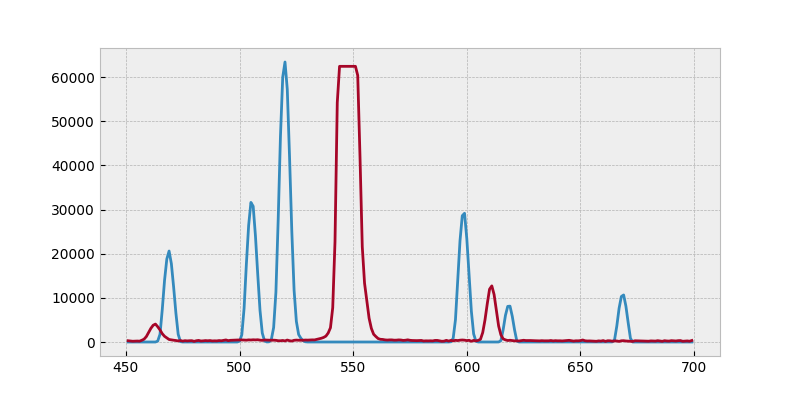
\includegraphics[height=.32\textheight, trim={1.2cm 0 17.5cm 5cm}, clip]{img/wl}
                    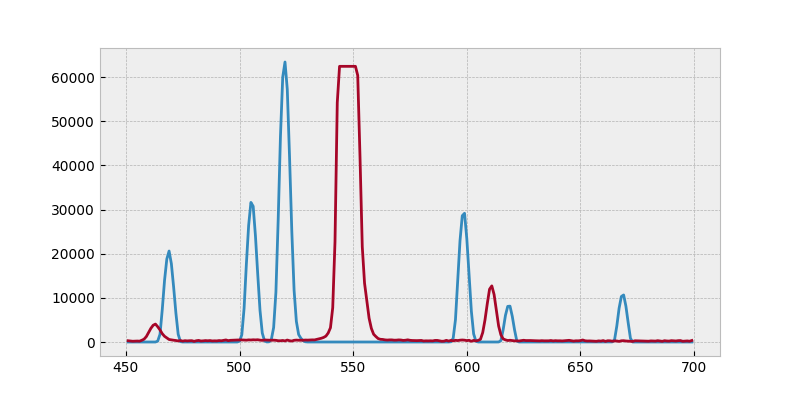
\includegraphics[height=.32\textheight, trim={10cm 0 5cm 5cm}, clip]{img/wl}
                    \caption{Intensit\"atsspektrum, um die unbekannte Linie}
                \end{figure}
            \end{minipage}
            \onslide<2->{
                \begin{minipage}{.65\textwidth}
                    \begin{align}
                        a_{uk} &= \SI{610.8+-4}{px}\\
                        \lambda_{uk} &= \lambdaUk\\
                        \nonumber\\
                        \lambda_{Th\ I} &= \lambdaTh\\
                        \lambda_{Xe\ I} &= \lambdaXe\quad \rightarrow \SI{0.38}{\sigma}
                    \end{align}
                \end{minipage}
            }
        \end{myframe}

  % !TeX root = ../pres.tex

\section{Zusammenfassung}

\end{document}
